%%%%%%%%%%%%%%%%%%%%%%%%%%%%%%%%%%%%%%%%%%%%%%%%%%%%%%%%%%%%%%%%%%%%%%%%%%%%%
%%%
%%% File: thesis.tex, version 1.9, May 2015
%%%
%%% =============================================
%%% This file contains a template that can be used with the package
%%% cs.sty and LaTeX2e to produce a thesis that meets the requirements
%%% of the Computer Science Department from the Technical University of Cluj-Napoca
%%%%%%%%%%%%%%%%%%%%%%%%%%%%%%%%%%%%%%%%%%%%%%%%%%%%%%%%%%%%%%%%%%%%%%%%%%%%%

\documentclass[12pt,a4paper,twoside]{report}         
\usepackage{cs}              
\usepackage{times}
\usepackage{graphicx}
\usepackage{latexsym}
\usepackage{amsmath,amsbsy}
\usepackage{amssymb}
\usepackage[matrix,arrow]{xy}
\usepackage[T1]{fontenc}
\usepackage{ae,aecompl}
%\usepackage{shortcut} %definitii pentru diacritice; 
\usepackage{amstext}
\usepackage{graphics}
\usepackage[T1]{fontenc}
\usepackage{ae,aecompl}
\usepackage{algorithm}
%\usepackage{algorithmic}
\usepackage{color}
\usepackage{color}
\usepackage{url}
\usepackage{listings}

\mastersthesis
%\diplomathesis
% \leftchapter
\centerchapter
% \rightchapter
\singlespace
% \oneandhalfspace
% \doublespace

\renewcommand{\thesisauthor}{Ioana-C\u{a}lina TUTUNARU}    %% Your name.
\renewcommand{\thesismonth}{July}     %% Your month of graduation.
\renewcommand{\thesisyear}{2016}      %% Your year of graduation.
\renewcommand{\thesistitle}{ATHENA - Aproach for Twitter Harvesting, Enhancement, Normalisation \& Analysis} 
\renewcommand{\thesissupervisor}{prof. dr. ing. Ioan Salomie}
\newcommand{\department}{\bf FACULTY OF AUTOMATION AND COMPUTER SCIENCE\\
COMPUTER SCIENCE DEPARTMENT}
\newcommand{\thesis}{MASTER THESIS}
\newcommand{\utcnlogo}{
\includegraphics[width=15cm]{img/tucn.jpg}}

\newcommand{\uline}[1]{\rule[0pt]{#1}{0.4pt}}
%\renewcommand{\thesisdedication}{P\u{a}rin\c{t}ilor mei}

\begin{document}
%\frontmatter
%\pagestyle{headings}

\newenvironment{definition}[1][Definition]{\begin{trivlist}
\item[\hskip \labelsep {\bfseries #1}]}{\end{trivlist}}



%\thesistitle                    %% Generate the title page.
%\authordeclarationpage                %% Generate the declaration page.

\pagenumbering{arabic}
\setcounter{page}{4}



\begin{center}
\utcnlogo

\department

\vspace{4cm}

{\bf \thesistitle} %LICENSE THESIS TITLE}

\vspace{1.5cm}

MASTER THESIS

\vspace{5cm}

Graduate: {\bf Ioana-C\u{a}lina TUTUNARU} 

Supervisor: {\bf \thesissupervisor}

\vspace{3cm}
{\bf \thesisyear}
\end{center}

\thispagestyle{empty}
\newpage

\begin{center}
\utcnlogo

\department

\end{center}
\vspace{0.5cm}

%\begin{small}
\begin{tabular}{p{7cm}p{8cm}}
 %\hspace{-1cm}& APPROVED,\\
 \hspace{-1cm}DEAN, & HEAD OF DEPARTMENT,\\
\hspace{-1cm}{\bf Prof. dr. eng. Liviu MICLEA} & {\bf Prof. dr. eng. Rodica POTOLEA}\\  
\end{tabular}
 
\vspace{1cm}

\begin{center}
Graduate: {\bf \thesisauthor}

\vspace{0.5cm}

{\bf \thesistitle}
\end{center}

\begin{enumerate}
 \item {\bf Project proposal:} {\it This approach combines time-proven unsupervised algorithms and specialised, state of the art text feature extraction with components of user-oriented business systems, to provide a solid but friendly decision support system of social media analysis. In essence, I present a process of data extraction that simplifies the task of analysing social media feeds, for business users and other stakeholders with little or no expertise in the domain of text feature extraction..}
\item {\bf Project contents:} {\it (Project Objectives and Specifications, Bibliographic research, Analyisis and Theoretical Foundation, Detailed Design and Implementa- tion, Testing and validation, User’s manual, Conclusions, Bibliography, Abbreviations and shorthand, Relevant code}
\item {\bf Place of documentation:} {\it Technical University of Cluj-Napoca, Computer Science Department}
\item {\bf Consultants:} Prof. dr. ing. Ioan SALOMIE
\item {\bf Date of issue of the proposal:} November 25, 2015
\item {\bf Date of  delivery:} July 5, 2016 {\it (the date when the document is submitted)}
  \end{enumerate}
\vspace{1.2cm}

\hspace{6cm} Graduate: \uline{6cm} 

\vspace{0.5cm}
\hspace{6cm} Supervisor: \uline{6cm} 
%\end{small}

\thispagestyle{empty}


\newpage
$ $
%\begin{center}
%\utcnlogo

%\department
%\end{center}

\thispagestyle{empty}
\newpage

\begin{center}
\utcnlogo

\department
\end{center}

\begin{center}
{\bf
Declara\c{t}ie pe proprie r\u{a}spundere privind\\ 
autenticitatea lucr\u{a}rii de licen\c{t}\u{a}}
\end{center}
\vspace{0.5cm}



Subsemnatul(a) \\
\uline{14.8cm}, 
legitimat(\u{a}) cu \uline{4cm} seria \uline{3cm} nr. \uline{4cm}\\
CNP \uline{9cm}, autorul lucr\u{a}rii \uline{2.8cm}\\
\uline{16cm}\\
\uline{16cm}\\
elaborat\u{a} \^{\i}n vederea sus\c{t}inerii examenului de finalizare a studiilor de masterat la Facultatea de Automatic\u{a} \c{s}i Calculatoare, Specializarea \uline{7cm} din cadrul Universit\u{a}\c{t}ii Tehnice din Cluj-Napoca, sesiunea \uline{4cm} a anului universitar \uline{3cm}, declar pe proprie r\u{a}spundere, c\u{a} aceast\u{a} lucrare este rezultatul propriei activit\u{a}\c{t}i intelectuale, pe baza cercet\u{a}rilor mele \c{s}i pe baza informa\c{t}iilor ob\c{t}inute din surse care au fost citate, \^{\i}n textul lucr\u{a}rii \c{s}i \^{\i}n bibliografie.

Declar, c\u{a} aceast\u{a} lucrare nu con\c{t}ine por\c{t}iuni plagiate, iar sursele bibliografice au fost folosite cu 
respectarea legisla\c{t}iei rom\^{a}ne \c{s}i a conven\c{t}iilor interna\c{t}ionale privind drepturile de autor.

Declar, de asemenea, c\u{a} aceast\u{a} lucrare nu a mai fost prezentat\u{a} \^{\i}n fa\c{t}a unei alte comisii de examen de licen\c{t}\u{a}.

\^{I}n cazul constat\u{a}rii ulterioare a unor declara\c{t}ii false, voi suporta sanc\c{t}iunile administrative, respectiv, \emph{anularea examenului de licen\c{t}\u{a}}.

\vspace{1.5cm}

Data \hspace{8cm} Nume, Prenume

\vspace{0.5cm}

\uline{3cm} \hspace{5cm} \uline{5cm}

\vspace{1cm}
\hspace{9.4cm}Semn\u{a}tura

\thispagestyle{empty}

\thispagestyle{empty}
\newpage

\begin{center}
\utcnlogo

\department
\end{center}

\begin{center}
{\bf
Cerere de elaborare a diserta\c{t}iei \^{\i}n limba Englez\u{a}}
\end{center}
\vspace{0.5cm}

Subsemnatul(a) \\
\uline{14.8cm}, 
legitimat(\u{a}) cu \uline{4cm} seria \uline{3cm} nr. \uline{4cm}\\
CNP \uline{9cm}, autorul lucr\u{a}rii \uline{2.8cm}\\
\uline{16cm}\\
\uline{16cm}\\
elaborat\u{a} \^{\i}n vederea sus\c{t}inerii examenului de finalizare a studiilor de masterat la Facultatea de Automatic\u{a} \c{s}i Calculatoare, Specializarea \uline{7cm} din cadrul Universit\u{a}\c{t}ii Tehnice din Cluj-Napoca, sesiunea \uline{4cm} a anului universitar \uline{3cm}, v\u{a} rog s\u{a}-mi aproba\c{t}i elaborarea lucr\u{a}rii de diserta\c{t}ie \^{\i}n limba Englez\u{a}.

Limba Englez\u{a} este de mare circula\c{t}ie interna\c{t}ional\u{a} \c{s}i prezint\u{a} bune oportunit\u{a}\c{t}i de discu\c{t}ie \^{\i}n comunitatea stiin\c{t}ific\u{a}. Doresc s\u{a} elaborez prezenta lucrare \^{\i}n limba Englez\u{a} pentru mai buna ei vizibilitate.

\vspace{0.5cm}

Data \hspace{8cm} Nume, Prenume

\vspace{0.5cm}

\uline{3cm} \hspace{5cm} \uline{5cm}

\vspace{0.5cm}
\hspace{9.4cm}Semn\u{a}tura

\vspace{0.5cm}
\hspace{8cm} \uline{5cm}

\vspace{0.5cm}
\textbf{Semn\u{a}turi aprobare:}

Profesor \^{\i}ndrumator: Prof. dr. Ioan SALOMIE: \uline{5cm}

\vspace{0.5cm}

\c{S}ef de catedra: Prof. dr. Rodica POTOLEA: \uline{5cm}

\vspace{0.5cm}

Decan: Prof. dr. Liviu MICLEA: \uline{5cm}

\newpage


%\listoftables
%\listoffigures

%\clearpage 
%\newpage

\newpage

\listoffigures
\tableofcontents
\newpage



\chapter{Introduction - Project Context}
\pagestyle{headings}

Not long time ago, big data and the need for content analysis were idealistic, intangible concepts. However, recent developments in computer performance and the growing popularity of social media has enhanced the need for novel academic approaches in this field.

The biggest challenge with processing these huge amounts of data lies in its sheer volume. This is highly problematic in many different ways:

\begin{itemize}
 \item storing and managing data is costly and sometimes needs special structuring attention
\item irregularities across data streams often indicate the need for extra transformations
\item filtering out noise and the extraction of meaningful data from thousands of entries requires specialised algorithms, architectures and platforms which are either inaccessible or difficult to use by regular users
\end{itemize}

\section{Project context}

Social media platforms these days have a strong presence in "the Cloud", which allows more and more developers to solve the problem of storage space and scalability in a relatively easy way. The high adoption of platforms like Facebook, Twitter, Instagram and many others have resulted in the generation of hundreds of thousands of online documents, text and media alike. Such a deluge of information is highly applicable for business purposes, but in is often stuck as a "diamond in the rough". An array of new and exciting job titles has also appeared, such as "Social Media Marketer", "Social Media Manager", "Social Media Expert" and so on. Not only do they represent career alternatives for a new generation, but they are also still outliers for decision support software.

\subsection{Social Media and why people care about what it says}

While the concept of Social Media is not a new one to be precise, it is clearly just starting to engulf us. The spread of Social Media alongside the spread of worldwide Internet access, the emergence of specialised applications and the recent shift to mobile online presence are objective realities. Subjectively as well, people have become more engaged to consuming, creating and sharing content online, which is evident in newspaper sales drops, app sales increase, events "going viral" within groups and even the online presence of a political critical mass. Companies offer barter possibilities for a variety of bloggers and vloggers to push products to their followers (which is not only more effective\footnote{http://www.techrepublic.com/article/election-tech-why-social-media-is-more-powerful-than-advertising/}, but also cheaper).

No wonder social media has a stake in public decisions! But for the first time in decades, people's choices are also quite open and public. Which means that some parties can get clues about society's preferences by using public data available on platforms such as Facebook, Youtube and Twitter. Consider two basic use cases, which I will emphasise throughout the course of this thesis:

\begin{itemize}
\item What does social media say about X?
\item What does social media say about X vs. Y?
\end{itemize}

where X and Y can be public people, events, brands, companies etc. 

\subsection{Data Analysis tools today}

There are a number of current platforms for data analysis, in the large sense including chart generators, format converters and importers and data visualisation plug-ins of sorts. Crossing into the realm of powerful analysis applications, most of them are complex and confusing to non-engineers, examples including Tableau\footnote{https://public.tableau.com/s/}, RapidMiner\footnote{http://rapidminer.com} and WolframAlpha\footnote{http://www.wolframalpha.com}. Figure \ref{fig:tableau} shows Tableau's interface, which may seem quite intimidating.

\begin{figure}[ht]
    \centering
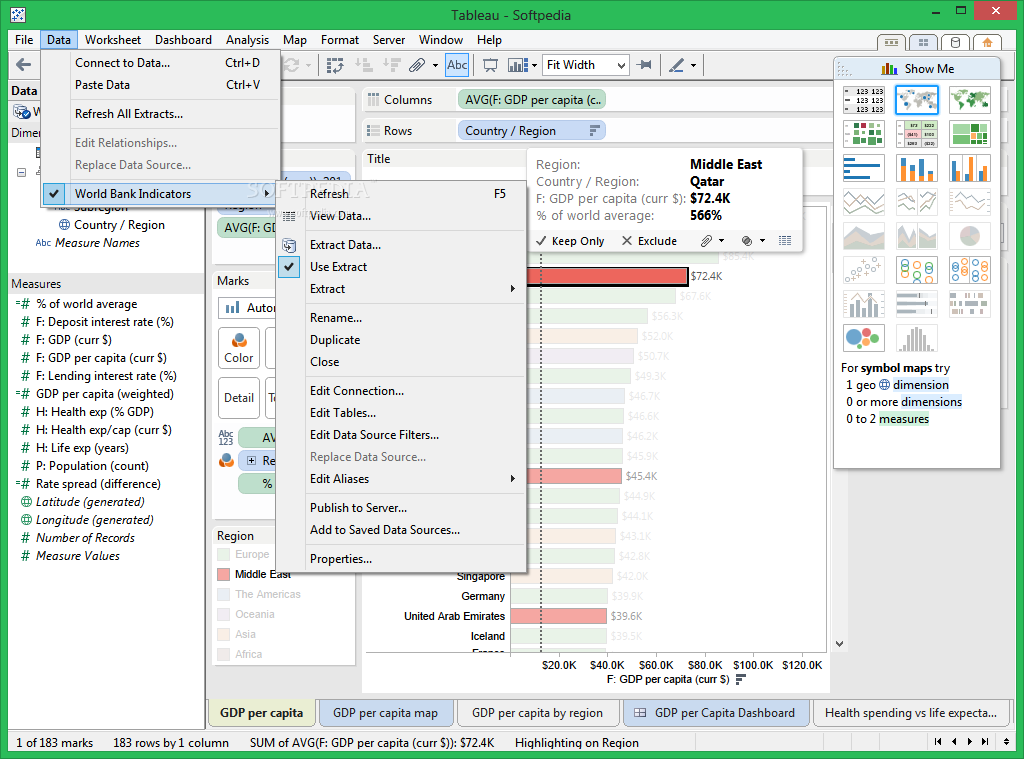
\includegraphics[width=0.8\columnwidth]{img/Tableau-Desktop_3.png}
    \caption{Tableau's interface}
    \label{fig:tableau}
\end{figure}

\subsection{Crossroads: Social Media in Business Intelligence}

The Computer Science field is very much branched nowadays in clearly-delimited subjects. But it is such a case where the large-scale processing capacities of data analytics should merge with approaches for computer-assisted business decisions. Consider that data analytics software often requires extensive training and a specialised knowledge, while most users desire only simple, straightforward functionalities for basic data analysis. One of Object Oriented Programming's fundamental principles is that of abstraction, in which end users need not (and should not) be aware of what is under the hood. Yet in data analytics, this is still the case on a 

The following Master's Thesis is the result of such an endeavour, to combine solid concepts from big data analysis, web application architecture and design, as well as enterprise software and economics for a better understanding of social media trends and opinions.

\subsection*{Thesis structure}
{\color{red} TODO
}

\chapter{Project Objectives and Specifications}
The project's purpose is to help non-expert users interested in social media analysis to get relevant and reliable information regarding specific concepts. 

\section{Web architecture}
A web architecture is preferable as a modern-day alternative to installable applications. The fast evolution of mobile devices has pushed web developers to segregate User Interfaces from Backend implementations, permitting devices to seamlessly connect to the same under the hood implementation without much development cost and overhead. Communication via REST services is crucial in this concern. Beyond user preference towards such applications, a web architecture presents even more advantages:

\begin{itemize}
\item virtually infinite space extensible with storage backends such as AWS3 or Google Cloud
\item scalability and outsourcing of time-costly services such as getting stream histories
\item database distribution over nodes
\item easily available documentation and integration throughout the development process
\end{itemize} 

Using a web framework eases development even more so and presents security advantages such as stable features, packages and quick patches in the odd case of a security breach. Plugging in services is also considered in the project's context, with handling of specific use cases done in separate managers, loosely coupled with the Model-View-Controller architecture.

\subsection{Data storage}
Since scalability and distribution are a must for a large-scale stream analysis project, data storage should be handled using a method which supports such breakdown while still remaining query-efficient. NoSQL databases are a popular choice for such implementation. The correspondence between the database storage backend and the model part of the application should also be loosely coupled, allowing for the possibility of switching between database backends if the need arises.

Big players in the field of non-relational databases are obvious possible choices: HBase, Cassandra, MongoDB, CouchDB, etc.

\section{ATHENA breakdown}
This thesis is based on the ATHENA original project, which comprises different pipeline steps in acquiring and analysing Twitter feeds:

\begin{itemize}
\item Harvesting: acquisition of collections of related Twitter statuses, by hashtag and dates (start and end).
\item Enhancement: basic analysis of a single harvest with classical unsupervised algorithms
\item Normalisation and Analysis: comparative analysis of harvests
\end{itemize}

\subsection{Twitter as data source}
For the development of this project, I chose to only implement one social media backend as data source. Twitter was the choice, since the character limit they impose is a great asset in regards of data processing: First of all, the classical data analysis pipeline deals with special cases such as documents of different lengths providing unusual skewing to the data set. Another advantage of Twitter is the prevalence of the hashtag model, which has failed to catch on with Facebook to the same degree. This means that statuses basically come out of the box already tagged for content.

Twitter is arguably the second most popular social media platform at the time, gaining on a large number of users even before the mobile device explosion, by integrating with telephone service providers to facilitate posting through SMS. Its 140 character limit makes for a good spin, which has pushed Twitter into a more textual realm than its more successful counterpart, Facebook. The platform is largely popular in the United States and especially in the entertainment domain\footnote{https://en.wikipedia.org/wiki/Twitter}, with the most popular Twitter accounts belonging to celebrities.

It notably also has a history of being the "go to" source for data analysis, after the United States' current president Barrack Obama purportedly used it in his 2008 campaign as one of the principal media outlets, choosing to have a strong Twitter presence, akin to advertisement presence of past candidates.

In short, although this approach is social platform-independent, Twitter was chosen even from the specifications step of this project for a clear start towards the data mining part.

\subsubsection{Fetching data through asynchronous jobs}
Since most social media platforms communicate with external applications via REST APIs with rate limits, the project's structure should include asynchronous modules. In this way, the user will be able to send an API-intensive job for queueing and asynchronous processing, without hindering their overall experience of using the application. This becomes apparent in the Harvesting part.

\subsection{Harvesting}
If we interpret ATHENA as a classical pipeline, then it becomes clear that the Harvesting part is the acquisition part. In order to perform analysis on data, it must first be fetched according to predefined rules and user options. Being time-intensive, these jobs must be designed asynchronously, following a FIFO model.

Figure \ref{fig:harvestpipe1} represents the conceptual model of data acquisition, starting from a collection of grouped documents (in our case they will be collections of statuses with a common hashtag). The Harvest manager handles sending asynchronous jobs via a FIFO queue towards a Consumer-type Harvesting job, represented as black box and further detailed in Figure \ref{fig:harvestpipe}. It is important to note that this pipeline is not in any way adjusted to the domain or the particular API platform; the only constraint we impose is that of periodically checking for compliance to rate limits. Social APIs usually limit requests either by number of requests or requested data size per unit of time. It is therefore a good idea to consider if any limitations alter our pipelines before starting on implementations.

\begin{figure}[ht]
    \centering
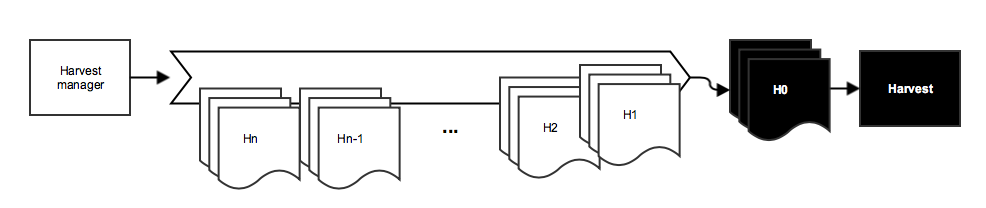
\includegraphics[width=\columnwidth]{img/harvestpipe1.png}
    \caption{Harvesting pipeline}
    \label{fig:harvestpipe1}
\end{figure}

\begin{figure}[ht]
    \centering
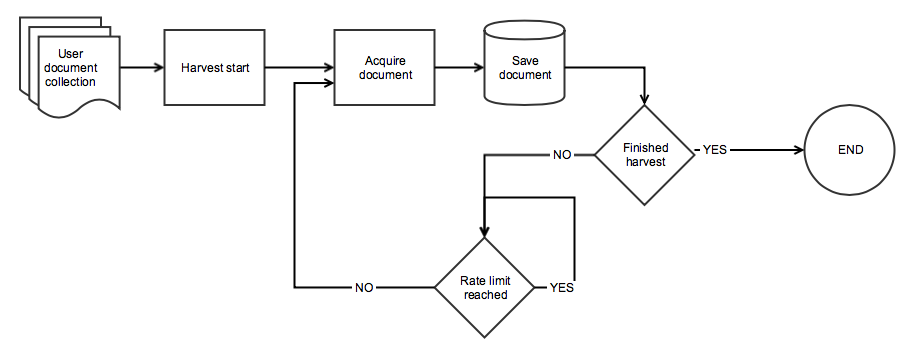
\includegraphics[width=\columnwidth]{img/harvestpipe.png}
    \caption{Harvesting job sub-pipeline}
    \label{fig:harvestpipe}
\end{figure}

\subsection{Enhancement}
As previously stated, it is not of great importance to have the data, but the goal is to obtain meaningful information from it. In this thesis I will refer to "harvests" as per the following definition:

\begin{definition}{}
A Harvest is a collection of documents related by contant, containing a token T and spanning from a start date and to an end date, which have gone through the harvesting pipeline and are stored for further anaylsis.
\end{definition}

After completing the Harvesting pipeline, resulting harvests are processed using various data extraction algorithms and presented to the user in the Enhancement step. These algorithms each have their own sub-pipelines of transformation, which will be detailed in the Analysis step.

\subsubsection{User contribution modeling}
{\color{red} TODO
}

\subsection{Normalisation and analysis}
{\color{red} TODO
}

\section{Non-functional requirements}
I am much concerned with the user's perspective in developing this application. As explained previously, one of the main objectives of this application is undoubtedly to be as simple to use as possible, to benefit non-expert users.

Firstly, I believe that a familiar and streamlined user experience should be implemented. The UI should have componenents found in most web application nowadays, in order to seem aproachable. The customisation options should also be loaded without input from the user, so that things like algorithm choices and parameters should stay hidden. Non-expert users do not know what \emph{Tfidf Vectorizer} or \emph{KMeans clustering} means, all they care about is to have some paplable results to their queries. In short, it is in the benefit of the non-expert users, which I target through this application, to have as little inputs, panels and buttons to figure out.

Besided the look and feel, users will also be interested in having a fast and reliable application. Exceptions and possible bugs should be properly filtered out and time-consuming jobs moved as per Figure \ref{fig:harvestpipe} to asynchronous jobs.
\chapter{Bibliographic research}

Although the ATHENA application itself is original work, it is common practice to reuse validated approaches and combine well-known algorithms to achieve a goal such ambitious as this one, i.e. to provide social media analytics capabilities in a familiar, web-based application, to non-expert users. A number of approaches related to this field are in existence, with some having overall structural similarities (e.g. pipeline approaches or web-based applications), while others being proven solutions for just part of the ATHENA pipeline (e.g. K-Means clustering, Power law fitting etc.).

\section{Social media analytics}
Social media analytics has received much attention in recent years. Since the explosion of social networks such as Facebook, Twitter, Instagram and others, the number of sentiment-loaded posts authored by individual users has increased exponentially. This raises the problem of filtering out useless data and noise, and compiling the large number of posts into useful, concentrated information snippets social media marketers can use for advertising and barter choice purposes.

\section{In-house social media}
Exploiting on the trend for social media data mining, some social networks have created their own analysis tools. Much of these are internal, but examples such as Facebook's Graph Search, which is free to use by application developers and individual users, are great tools for analytics purposes. Approaches such as the 2014 study \cite{spirin2014people} found that using Facebook Graph Search can facilitate people search along demographics and profiles.

Besides in-house tools, social media networks provide APIs for developers interested in researching user behaviour, brand popularity etc. Examples include Facebook, Twitter, Instagram, LinkedIn, Pinterest, Foursquare, Meetup, Slack, Flickr and Google Plus\footnote{http://www.programmableweb.com/news/top-10-social-apis-facebook-twitter-and-google-plus/analysis/2015/02/17}. Web mining approaches such as \cite{java2007we} try to understand virtual social communities by using these APIs. This latter study uses Twitter API. It is not surprising that the reusability of certain API queries were exploited in numerous API wrappers, in different programming languages\footnote{https://dev.twitter.com/overview/api/twitter-libraries}.

\subsection{Social media analytics in companies}
Enterprise resource planning (ERP) systems appeared in the 1990s as a counter wave to company siloing. The phenomenon is described as the specialisation and lack of streamlined cooperation between company departments. Marketing is one such department, in which operations should take into account results and goals from other departments and external sources combined. Unfortunately, since the social media explosion took place in recent years only, and ERP systems are generally large-scale and quite resistant to change, it is yet not implemented that social media data mining tools are well-integrated in ERPs. This is in spite of the clear connection between social media and Web 2.0 concepts to retailing power, as proven by numerous studies \cite{constantinides2008social}.

\section{Structurally-similar works}
The following section presents the advantages and drawbacks of using meta-frameworks such as approaches to application development and natural language processing.

\subsection{Advantages of web applications}
Web applications enjoy a high popularity since it is not necessary to install any software on computers in order to run such applications. Almost all modern computer users use web browsers, and so the execution intermediary is already installed in most cases. Ease of usage without downloading anything, availability of updates and patches without any distribution chain necessary and other advantages as mentioned in \cite{tung2013internet} suggest the appropriateness of developing such an application as a web one. Another important advantage is the fact that in case users develop a need to run this application from mobile devices, a REST architecture to expose the modules would suffice.

Since web application frameworks are ubiquitous these days, it is also the case that a scientifically-rich Python application can easily be integrated to a web application using one of Python's frameworks such as Django, Flask or CherryPy. Indeed the number of wrappers and tools available in Python's scientific libraries have prompted researchers to make various natural language processing applications in this language. The 2009 book "Natural language processing with Python" \cite{bird2009natural} encourages developers to use Python as a programming language most suitable for text processing, complete with support from external libraries such as NLTK (Natural Language ToolKit), Sci-Kit Learn (for machine learning), SciPy, Numpy, matplotlib and so on.

We conclude that the prevalence of the Python recommendation in literature is significant in making a decision related to the project's development. Based on numerous similar approaches, ATHENA also employs Python and its web application components in creating an easy to use and relevant social media analysis tool.

\subsection{Pipeline model}
Pipeline model-based applications are mostly common in the text processing domain of research. The approach works well for large data sets since it is difficult to transform the data end-to-end in one go. The specialised modules which compose the pipeline are indeed fitting with the general concepts of SOLID Object-Oriented Programming, since pipelines respect:

\begin{itemize}
\item \textbf{S}ingle Responsibility - each module handles one type of simple transformation
\item \textbf{O}pen Closed - each module collaborates with its neighbours in the pipeline using interfaces
\item \textbf{L}iskov Substitution - modules are interchangeable, in the sense that you can code to an interface and change each particular type of module with a similar one
\item \textbf{I}nterface Seregation - pipeline steps are loosely coupled and generally do not depend on specific methods from unrelated steps
\item \textbf{D}ependency Inversion - the building blocks are usually stable components
\end{itemize}

Futhermore, the usage of pipelines in natural language processing, data mining and other text-related endeavours, is time-proven, with renowned research groups adopting it as a general principle. One of such groups is the Stanford NLP Research Group \cite{manning2014stanford}. The wide-spread practice became even more popular when text feature extraction (e.g. GATE, LaSIE, IXA, LONI etc.) tools adopted the same principle. Figure \ref{fig:nlpipe} presents a pipeline implementation used by some applications which handle text processing.

\begin{figure}
    \centering
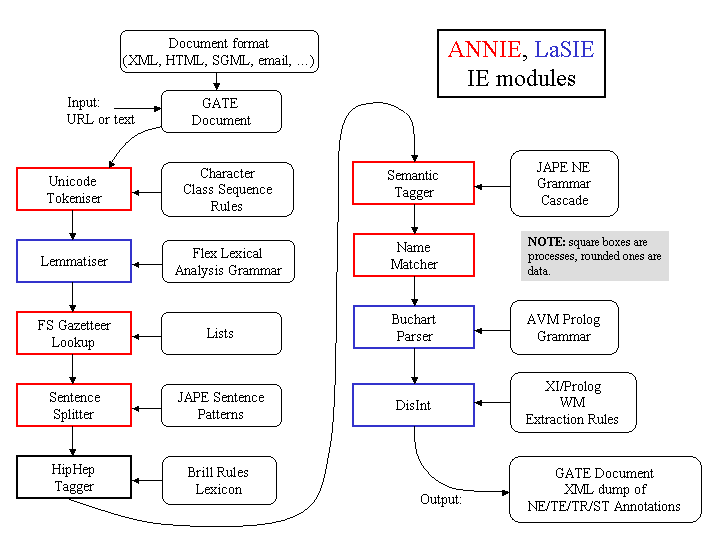
\includegraphics[width=0.8\columnwidth]{img/annie-pipe.png}
    \caption{Classical NLP Pipeline as applied in ANNIE and LaSIE text processing tools}
    \label{fig:nlpipe}
\end{figure}

ATHENA's pipeline is similar in the sense that it prepares the document set during the Harvesting step, then it Enhances the dataset with useful data. The third pipeline step is normalising (or flattening) the data set to its most useful and representative core, while the final step takes as input the normalised document sets and runs a comparative Analysis.

\section{Data modeling and extraction approaches}
The vast domain of text feature extraction and text mining is a very diverse one. A variety of approaches can be applied, as discovered by many branches of research. One of the most important issues to discuss is the advantages and drawbacks of the domain-related and domain-independent categories of machine learning, and what they mean for natural text processing. Towards the end of this section, the discussion will move to scientifically sound and time-proven methods which achieve parts of the necessary functionalities in ATHENA.

\subsection{Supervised vs. unsupervised learning. Domain vs Domain-independent approaches}
As previously discussed, one of the biggest discussions to be had at the start of a text processing application's development, is whether the application will fall into either one of the categories: supervised vs. unsupervised machine learning, domain-related or domain-independent. Usually the categories are coupled in the sense that domain-independent data can not be correctly processed within a supervised approach, which means the two are incompatible.

Supervised learning starts from the premise that we can classify some existing, annotated data, and once the classifier is correctly trained, it can be launched onto the real, full-scale dataset and perform well. Indeed with supervised learning, considering the domain-related approach, an impressive accuracy rate can be obtained. Factors such as the training set size, completeness and correctness influence, along with domain-specific tweaks, can combine to create a powerful classifier. However, there are some drawbacks: 

\begin{itemize}
\item the approach can not be generalised to other domains without existing annotated data for those domains
\item the training set is often difficult to find  and/or manually annotate. Such a training set requires a lot of resources and a dedicated staff, while for the best final accuracy the number of documents correctly labeled in the training set should be very large.
\end{itemize}

Applications such as ATHENA seem to not have a choice but use the domain-independent approach, with specifically domain-independent algorithms to build the analysis results. But the results in the field are not discouraging. In 2002, a study by Turney \cite{turney2002thumbs} found an accuracy rate of 74\% for an unsupervised learning approach, applied to text processing and sentiment analysis in particular. ATHENA does not restrict limits on the hashtags users can use to build harvests, and is in the impossibility of building training sets for all such hashtags, so it falls into the area of unsupervised learning. It is important to note that subsequent algorithms for calculating various application analysis results should therefore also be unsupervised ones.

\subsection{Clustering}
One of the most important unsupervised learning concepts that ATHENA uses, both in the Enhancement and Analysis steps, is that of clustering. Clustering is the grouping of related document features and/or documents, based on common features. It does not require any training data as input and does not have specific domain applicability, which means it is safe to use throughout our application.

A Google Scholar search of the terms "document clustering" produces almost 1.5 million results in books, papers and conference proceedings. The prevalence of clustering algorithms is due to it's easy to understand process and applicability over a large range of possible datasets. A 2000 study by Steinbach et. al \cite{steinbach2000comparison} compares the accuracy of some clustering algorithms, including:

\begin{itemize}
\item K-Means
\item bisecting K-Means
\item UPGMA (Unweighted Pair Group Method with Arithmetic Mean)
\end{itemize}

with different centroid calculation methods. It demonstrates that bisecting K-Means performs best for hierarchical clustering, with some dataset particularities constituting exceptions.

\subsubsection{KMeans}
The clustering algorithm used in ATHENA is K-Means. Initially proposed by Stuart Lloyd in 1957 and applied to research in pulse-code modulation\footnote{https://en.wikipedia.org/wiki/K-means\_clustering}, K-Means has become popular in cluster analysis and data mining after its republication in Fortran by Hartigan and Wong in 1975/1979, which featured better efficiency. The algorithm starts from a number of K centroids and then alternates between two types of steps:

\begin{itemize}
\item assignment: assign each data point to the nearest centroid (in Euclidean distance)
\item update: calculate new centroids at the mean of points assigned to each centroid
\end{itemize}

KMeans runs these steps alternatively until convergence, which is achieved when centroids no longer move from iteration to iteration, or at least do not move over a distance greater than a predefined minimum.

ATHENA uses a variant of KMeans which translates the term occurrence and frequency in the document set to Euclidean distance, i.e. the presence of common terms inside a pair of documents defines the closeness of those documents.

\subsection{Power law dataset analysis}
Another important issue we need to correctly handle is the modelling of users behaviour in authoring documents. We are mostly interested in the degree of fitting of post numbers per user to the existence of a power law. Perhaps one of the best-known example of a power law in effect is that proposed by the Italian economist Vilfredo Pareto, that 80\% of the land in Italy was owned by 20\% of the population. The extension to other fields soon became apparent, with Pareto's law being generalised as: "For many events, roughly 80\% of the effects come from 20\% of the causes\footnote{https://en.wikipedia.org/wiki/Pareto\_principle}. When applying Pareto's law to our dataset of document numbers, it might be the case that unusually high numbers of documents are authored by unusually low numbers of users.

In Nassim Nicolas Taleb's 2007 book "The Black Swan"\cite{taleb2007black}, the principles of power laws are given great focus. The author maintains that the existence of power laws in economic contexts is of such nature, that the modeling of economic events in Gaussian distributions is entirely wrong, with Mandelbrotian (fractal) modeling being far more suitable. The argument is that, in such datasets, the outliers are so powerful, that they skew the results of an otherwise correct calculation. These long tail measures apply mostly to data which is not a physical property such as height or weight of people, but to economic and social aspects such as popularity, wealth, career-wise success. It is probably safe to admit that post numbers and post popularity in social media fall into the same non-physical category which can many a times be modeled as a power law distribution.

As to calculation methods of this fitting degree, authors Clauset et. al built a Matlab implementation of an algorithm doing these estimations. The formal proof of algorithm correctness, as well as arguments for the algorithm, are collected in a 2009 study \cite{clauset2009power}. The same algorithmic approach was later translated to various programming languages either by the authors themselves, or by third party developers interested in using the library. These endeavours saw R, Python, C++ and Java libraries created on the same basic ideas.

\subsection*{Summary}
In this chapter I discussed the similarities between the proposed application of ATHENA and other scientific endeavours to create feature extraction systems. The subjects covered started with arguments for designing ATHENA as a web application and using the pipeline architecture, as validated and widely-used throughout the scientific community concerned with text processing.

I then discussed the advantages and drawbacks of domain-related vs. domain-independent text processing, as well as the supervised and unsupervised approaches, motivating why only the latter is suitable for the ATHENA application and explaining the consequences of this categorisation. In the last part of this section, I covered a couple of algorithms used in the analysis the application performs, with KMeans and Plfit as algorithms suitable to unsupervised learning and thoroughly researched and validated by the scientific community.

More in-depth analysis of existing approaches, their suitability to this project and particular implementations needed will be discussed in the next chapter
\chapter{Analysis and Theoretical Foundation}
\label{ch:analysis}
While the previous chapter covered existing theoretical approaches which intersect somewhat to the ATHENA approach itself, the following will go into more detail related to scientific methods used throughout the application. The theoretical foundations of ATHENA will be covered, with the conceptual behaviour of such an application being formally described. Please note that the following set of methods apply to a variety of text feature extraction use cases and are not in any way bound to the application itself, but rather belong to the general approach. For details on the implementation of the ATHENA approach as implemented in a Django/Python web application, consult Chapter 5 of this thesis.

\section{Pipeline architecture}
Pipeline architectures are an idea emerged at the dawn of the industrial era to better manage the production cycle of factories. The basic idea is that workers are specialised and only perform small parts of the total work needed to complete a task or project, with the semi-finished goods being transported between specialised stations throughout the process.

These concepts were first applied in computer sciences in the context of pipelined CPUs\footnote{Central Processing Unit} with the aim of increasing instruction number per unit of time. This meant executing the micro-instructions separately, storing the result and reusing that stored result as message exchange between the pipeline steps. Figure \ref{fig:cpupipe} presents a classical RISC pipeline with 5 steps: Instruction Fetch, Instruction Decode, Execute, Memory access and Register write back.

\begin{figure}
    \centering
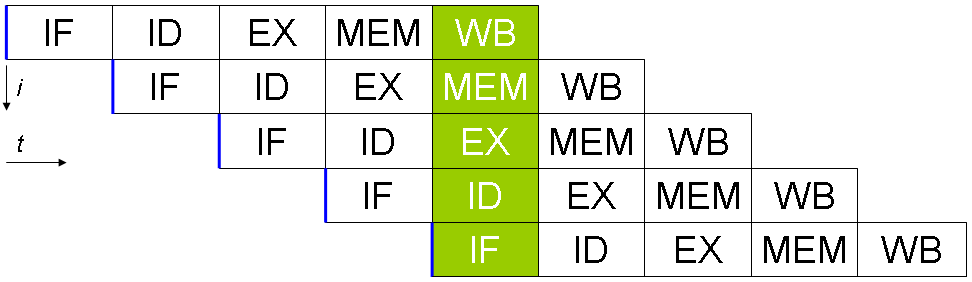
\includegraphics[width=0.8\columnwidth]{img/cpupipe.png}
    \caption{Five-stage pipeline in a RISC machine}
    \label{fig:cpupipe}
\end{figure}

As discussed in the previous chapter, the pipeline architecture has subsequently gained momentum in high-level computing as well. The pipeline architecture is suitable for projects which feature large transformation efforts with multiple failure points. By separating the set of transformations into separate steps, the black boxes composing the broken down architecture are separate entities with manageable numbers of failure points. Furthermore, the communication between the black boxes takes place by using stored semi-finished data as a method of message exchange.

Pipeline architectures are well suited for Object-Oriented Programming best practices as well, since the concept itself is SOLID (Single Responsibility, Open/Closed, Liskov Substitutional, Interface Segregated and Dependency Inverted, as per previous chapter discussion). The architecture is also encouraging of loose coupling and scaling to distributed applications. Considering the task of developing applications for fetching and analysing data from social media, it is self-understood that scaling towards distribution might be mandatory from some point on.

\subsection{Black boxes}
In the context of this approach, the black boxes which correspond to different pipeline stages are:

\begin{itemize}
\item the Harvesting module: methodology and system of fetching data from external APIs provided by different social networks.
\item the Enhancement module: methodology for enhancing the fetched and stored data with specific details which model its structure and particularities
\item the Normalisation module: handles the flattening of fetched and stored harvests using different configurations. This module helps filter outliers, noisy and/or erroneous data points, in the end storing the result.
\item the Analysis module: performs comparative analysis of differences and commonalities between already normalised data sets, with focus on differences and commonalities between the two
\end{itemize}

\subsection{Communication between modules}
The execution of the Harvesting module results in the fetching and storage of related document sets. These collections of documents are stored using a persistent and manageable data source. For the time being, the choice of the data source backend is unimportant, especially from a formal point of view. However, it must be noted that the data source to be chosen is required to be fast, scalable and easily manageable.

The communication from Harvest to Enhancement and Normalisation respectively is one much similar to the classical approach of pipelined CPUs, i.e. the data is stored and then recollected inside the destination modules. As it will be seen in further sections, the nature of asynchronous jobs (employed in order to fetch the data in rate-limited APIs) adds an extra buffer to this ad-hoc message exchange channel, by not permitting yet incomplete harvests to enter processes such as Enhancement and Normalisation.

Enhancement is a module without side-effects, which means the data it uses as part of calculations remains unchanged. However, it is another case when discussing the Normalisation module. The calculations of data flattening done by the Normalisation step are recorded in the persistence layer, for further use in the Analysis module.

Last but not least, the final step considers the data previously saved by the Normalisation step to make comparative calculations of similarity and differences between two document collections which have already passed through the Harvest and Normalisation steps and are now both:

\begin{itemize}
\item correspondent to real-life documents authored by users using the queried social network

\textbf{and}
\item flattened in order to eliminate outliers and noise.
\end{itemize}

Data is generally considered as output from source boxes (steps) and input for destination ones. This is easily enforceable using step-wise validation.

\section{Asynchronous application behaviour}
The following section covers the particularities of the Harvesting module, which necessitates special attention in regards to the execution of processes. I will cover the particularities of asynchronous jobs and why it is necessary to place part of this module inside such a job.

\subsection{Asynchronous jobs}
An important classification in regards of job execution in web applications (and not only) is whether the execution is synchronous or asynchronous. A synchronous job receives its input from the end user via the application, it executes and returns a result instantly, which the user waits for and gets immediately. In the case of asynchronous jobs, users send their input to the application, but instead of waiting for a response to come, they continue to browse, interact with the application and maybe even send more and more jobs to execute. On the backend side, said jobs are executed and might or might not notify the user when they have finished.

In dealing with large response times, it is generally better to use asynchronous execution, for a variety of reasons which culminate with the user's general experience. If a user is forced to wait for a result and prevented from doing anything else, they get easily frustrated. The ATHENA methodology, in particular the Harvest module, requires extensive querying of external data sources. Furthermore, the external APIs provided by social networks enforce rate limits, which means the client application can only get a maximum number or total size of documents before needing to sleep until the limit is replenished. It is impossible in this context to make the user wait for the result.

\subsection{Job handling with the Producer/Consumer architecture}
Up to now, we established the need for an asynchronous job execution as part of the Harvest module. To clarify on that, it is needed to establish a general architecture in which these jobs are created, executed and finalised.

\begin{figure}
    \centering
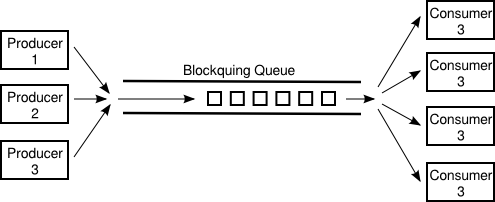
\includegraphics[width=0.8\columnwidth]{img/producer-consumer.png}
    \caption{Producer/Consumer architecture example}
    \label{fig:prodcons}
\end{figure}

The Producer/Consumer concept subsumes problems, architectures and design pattern suggestions throughout the computer science field, starting from the didactic example of the need to introduce semaphores and atomic operations in computer architecture. As a job execution framework, this setup is formalised as such:

Two processes called Producer and Consumer are connected using a buffer, which usually takes the form of a Blocking Queue. The Producer is tasked to generate data, add it into the buffer and start over. Meanwhile, the Consumer is removing data from the buffer (piecewise and in the order it was produced). In the context of asynchronous job execution, the Producer is the one that creates the jobs, while the Consumer handles each job, in order. Figure \ref{fig:prodcons} contains a graphical representation of these details.

ATHENA includes a Producer-Consumer architecture inside its Harvest pipeline, as part of the asynchronous job execution whose necessity was explained above. While the task of getting the options from an end user and creating the job setup itself should be part of a core system, the jobs are then sent via a buffer towards a Consumer. The Consumer is instructed to fetch the related document sets as per the read options from the buffer. As part of the Consumer, a social network's REST API will be used as a source for the document collection.

To clarify, the asynchronous functionality is provided by the Consumer. Indeed the buffer is also outside what we consider core synchronous functionality, but its just a passive data source.

\section{REST API communication}
As discussed in the previous chapter, social networks have not only developed in-house analysis applications, but moreover exposed APIs (Application Programming Interfaces) which developers can use in order to query for documents authored by users of that social network. Previous sections have described \emph{how} Harvesting works, but not exactly \emph{what} it does, i.e. the executable content of the Consumer.

Most APIs follow the REST architecture, which stands for Representational State Transfer. The method is widely-used as opposed to other Application service implementations, because of its compatibility between applications written in different programming languages and its general ease of use, which is based on calling URIs with one of the classical HTTP verbs:

\begin{itemize}
\item GET: to read data
\item POST: to modify data
\item PUT: to update by replacing data
\item PATCH: to update/modify data
\item DELETE: to remove data
\end{itemize}

REST services are called by a \emph{client} and affect a \emph{server}. In order to acquire data about users and posts from an API exposed by a social network, ATHENA assumes the role of a client in the exchange with the social network's servers. Usually since this approach works by fetching data and not modifying it, the primarily used verb is GET, along with different parameters.

\subsection{Authentication}
External APIs usually provide users with a variety of access tokens and/or secret codes which serve both to protect the API from illegal usage by identifying the client application and cutting off its access in case any irregularities are found. On the other hand, the client can make sure that, if they haven't distributed the access tokens to other parties, their account is safe from outside penetration, i.e. other clients can not impersonate the application to piggypack any requests.

These authentication details are usually sent in every request or otherwise the credentials are established once in a certain interval of time. In any case, for the examples below detailing the usage of HTTP methods and parameters in fetching social data, we oversee authentication description for simplicity purposes.

\subsection{Filtering with parameters}
When filtering the set of posts we are interested in, we consider input from the end user of ATHENA. They are not interested in getting all the posts of all the users in every time. However, the details provided by the user when creating the Harvesting job can be used in order to filter the request to only contain conformant data.

GET parameters can be directly added to the URL called on the server, by adding a question mark character at the end of the base URI (?) and adding key and value pairs of the desired parameters separated by ampersands (\&). The pairs themselves take the form:

\[key=value\]

ATHENA filters content by its label (content or, in the specific case of Twitter, hashtag) and date limits (start and end dates), which means the query URL will look something similar to:

\[https://api.twitter.com/1.1/search/tweets.json?\]
\[q=\#python\&since=2016-06-06\&until=2016-06-07\&lang=en\]

\subsection{API wrapper libraries}
It is worth mentioning that in often cases, the same type of requests are used by many developers. The repetitive nature of the task to be implemented creates the business value for API wrappers, which can seamlessly be used by developers, based on some input access keys and wrapper functions.

It was previously discussed throughout this thesis that external APIs usually enforce rate limits. These can usually take the form of maximum number or size of responses per unit of time. The solution is sometimes to halt the processes fetching the data until the rate limits are replenished. These is another very common use case with repetitive nature, which makes it a candidate for wrapper functions as well. In Chapter 5 we describe the activity of chosing an implementation method for these concepts, factoring in the benefits of API wrapper libraries and functions.

\section{Vectorising the data space}
As part of the Enhancement step, ATHENA is mostly concerned with structural particularities of the document sets. In other words, we are interested in modeling the most common occurrences of content, the most popular labels and categories assigned by authors and the general correspondence between users, their posted documents and their creative content.

A first step in achieving content analysis is to perform term ocurrence analysis. This step is often called \emph{vectorising} the collection of text documents, since it takes as an input the set of documents (as arrays of terms) and outputs a $m \times n$ matrix of term occurrences, where:

\begin{itemize}
\item $m$ is the number of rows i.e. text documents in the collection
\item $n$ is the number of columns i.e. tokens found (also known as terms, however the notion of token is used since the terms are intended as single-piece elements, with eventual corelations being studied later)
\end{itemize}

But what do we consider to be a token? Well, for the first iteration of this approach, the decision to use hashtags was a result of their prevalence throughout various social networks. This particular type of labeling is done directly by the user with special characters and has gained momentum ever since its introduction on Twitter, Instagram and later Facebook. Hashtags are therefore informal labels and/or categories, which transforms this otherwise unsupervised task of feature extraction into one of less difficulty, since users themselves have performed a sort of annotation.

A larger discussion about the usage of hashtags in the particular context of Twitter can be consulted in the next chapter. For now, suffice it to say that the vectorisation can consider only particular forms as tokens and can ignore non-hashtag content if instructed so.

\subsection{Sparse matrices}
Special attention needs to be dedicated to the result of the vectorisation step. Indeed the result is a matrix but considering the large number of documents and the little number of re-occurring terms one document may contain, the matrix will undoubtedly have many 0 values. Such a matrix is called \emph{sparse} and it requires special data structures and algorithms for proper processing. For example, consider the following document set:

\begin{enumerate}
\item The \#cat in the \#hat.
\item The \#hat in the \#flat.
\item The \#flat \#data set is better for \#analysis.
\end{enumerate}

Considering hashtag-only vectorisation i.e. only for tokens starting with the character "\#", it produces the following result, with columns from top to bottom: \#cat, \#hat, \#flat, \#data, \#analysis and documents from left to right 1, 2, 3:

\[ \left( \begin{array}{ccc}
1 & 0 & 0 \\
1 & 1 & 0 \\
0 & 1 & 1 \\
0 & 0 & 1 \\
0 & 0 & 1 \end{array} \right)\] 

With only 3 documents the resulting matrix is already somewhat sparse (containing 8 zero values to 7 non-zero ones), but considering a much larger document number, it becomes clear that a high proportion of the resulting matrix will contain zero values.

Generally a sparse matrix can be stored in different ways, including the classical two-dimensional array. However, traversing and modifying such a large data structure is considered cost-ineffective. Other formats\footnote{https://en.wikipedia.org/wiki/Sparse\_matrix} include those optimised for modifications:

\begin{itemize}
\item dictionary of keys: maps $(row, column)$ pairs to the value of elements
\item list of lists: stores one list per row
\item coordinate list: stores $(row, column, value)$ tuples
\end{itemize}

While other formats support efficient access and matrix operations:

\begin{itemize}
\item compressed sparse row: similar to coordinate list, but compresses the row indices. Indicated for row access and vector multiplication
\item compressed sparse column: similar to compressed sparse row but with columns compressed. Recommended for arithmetic operations and vector products
\end{itemize}

The exact type of storage used depends on the implementation itself. Some processing methods may produce one type of representation or another, but the underlying data structure will always be a sparse matrix. Having performed vectorisation, it is then a matter of calculations and choosing the correct algorithms towards the goal.

Vectorising the space and calculating clusters (as discussed below) are important parts of the Enhancement step in ATHENA.

\section{Clustering with KMeans}
While mere presence or absence of terms inside a document collection is interesting to consult, it is not a detail which gives users much information about the composition of said document collection. Vectorisation of terms is in this case a precursor for the clustering step, which uses the previously generated sparse matrix for identifying commonalities between some documents.

By clustering we generally refer to an approach, algorithm or general endeavour which assigns data points to agglomerations called clusters. The basic example follows points on a plane with given coordinates. Clusters of will be formed based on data points agglomerations, considered by the Euclidean distance measurement.

\begin{figure}
    \centering
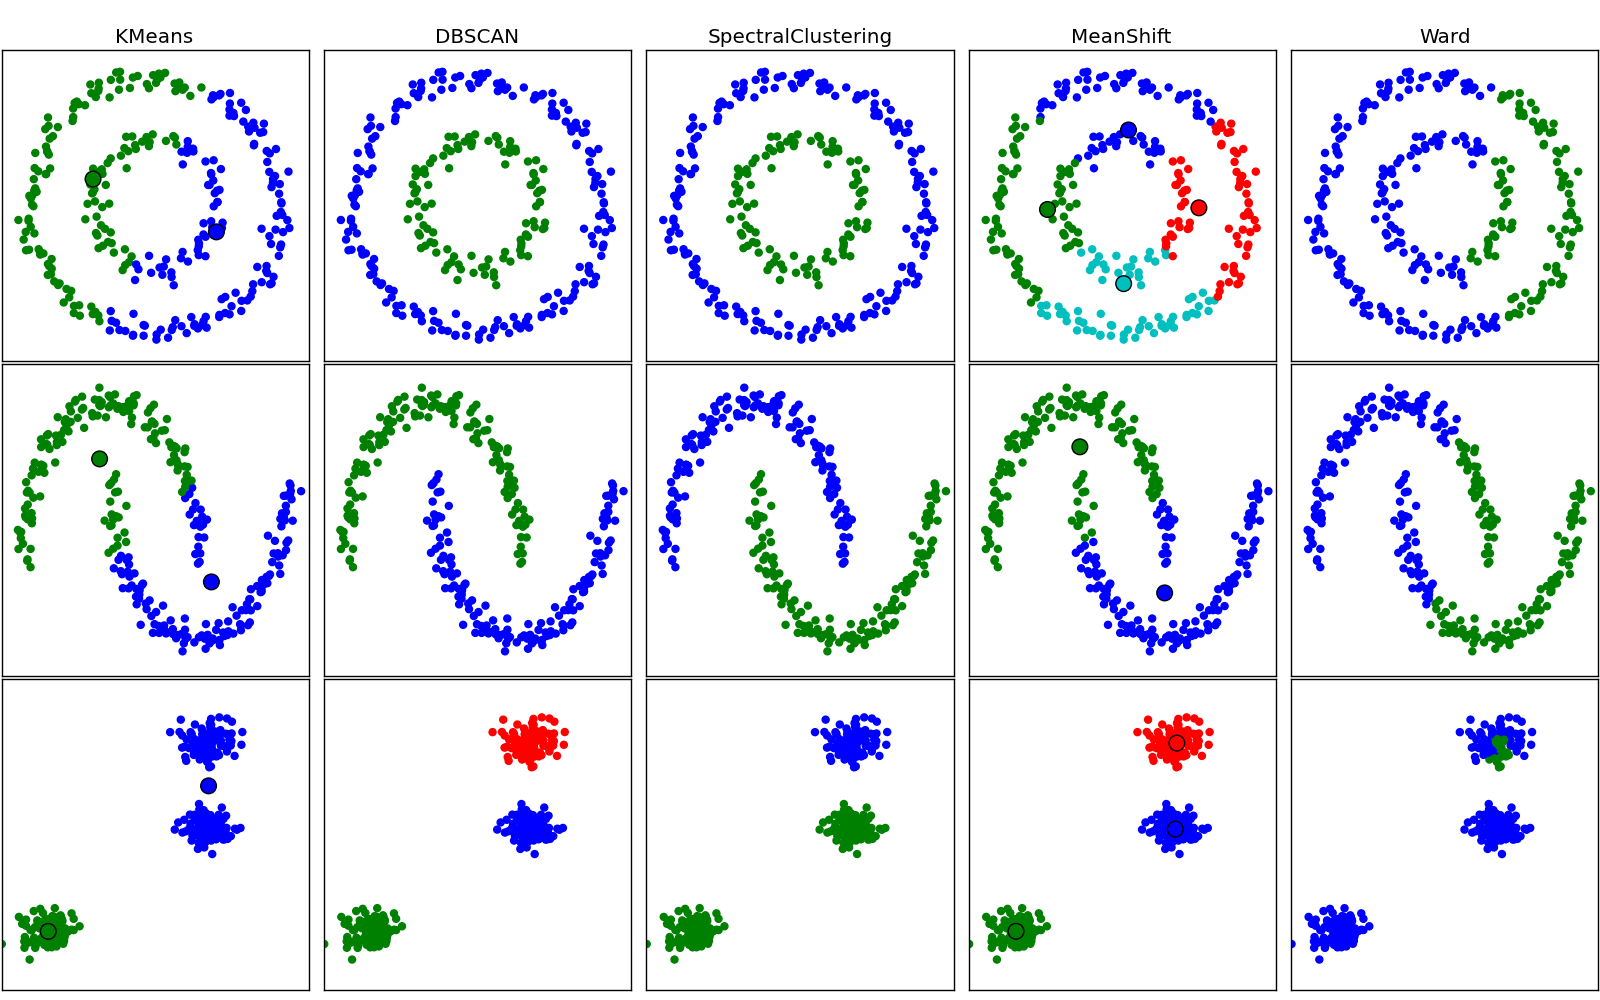
\includegraphics[width=\columnwidth]{img/clustering.png}
    \caption{Clustering algorithms in effect on various data sets}
    \label{fig:clustering}
\end{figure}

A variety of clustering algorithms exist, all with specific advantages and disadvantages. Some algorithms perform better on pattern-full data, while others handle unexpected metrics better. The efficiency of a clustering algorithm depends on the data particularities, initialisation and running options. Figure \ref{fig:clustering} exemplifies the performance of various clustering algorithms on different data sets, with data points marked as belonging to certain clusters by coloring on the graph. Note that some algorithms also place \emph{centroids} (represented in the figure as small circles) which represent the center of a cluster, although it doesn't necessarily coincide with a data point.

When considering term occurrence, clearly the distance is not the Euclidean classical one. However the distance in use here is the commonality of terms used throughout the document space. E.g. documents which are used in many documents together are considered \emph{close} while terms which never intersect inside the same document are \emph{far} from one another. Considering the general lack of irregularities and patterns possible inside a textual dataset, the K-Means algorithm is a good fit to our approach.

Essentially, the algorithm works by initialising a number of $k$ centroids and subsequently changing the cluster location and the data point assignment based on mean distances, i.e. at every execution step, a point is assigned to the closest centroid and a centroid's position is recalculated at the mean of its components. I will not go into much detail regarding the steps here, but rather into the problem of centroid initialisation and KMeans variants available.

\subsection{Centroid initialisation}
Centroid initialisation is a sensitive problem when considering K-Means algorithm implementation due to the propagation of errors and convergence time costliness an inappropriate initial setup could produce. The goal of centroid initialisation algorithms is to minimise intra-class distance (sum of Euclidean distances between each data point and its centroid). Some common centroid initialisation methods are:

\begin{itemize}
\item Forgy: randomly chooses k data points and uses them as initial means
\item Random partition: starts by randomly assigning a cluster to each data point
\item KMeans++: works by selecting an $i$ centroid using a probability function based on the minimum distance from an initial $x$. This algorithm usually prevents accidental selection of close centroids, which can propagate and affect the algorithm's working. Using a KMeans++ initialisation, it is guaranteed that the algorithm will converge in O(log k)
\end{itemize}

In order to ensure fast convergence to a good solution, the KMeans++ initialisation algorithm is a good fit for the approach presented in this thesis.\label{kmeansplusplus}

\section{Power law fitting}
In Chapter 3 I discussed the particularities of data sets which correspond to power functions. In this section I will ellaborate on the usage of these modeling techniques to identify potential pages, bots and fake accounts on social media. In concernes related to power functions and fractalic modeling, it is not problematic to output a data set corresponding to a power function, but I will present an algorithm handling the reverse problem: how, given a data set, we can calculate the degree to which it corresponds to a power law.

\subsection{Power functions and well-known examples}
\label{plfittheory}
In Chapter 3 I briefly mentioned Vilfredo Pareto's now famous law which stated that 80\% of the effects are generally the results of 20\% of actions, as well as other scientists' (such as Mandelbrot and Taleb) concerns towards understanding and modeling general power law principles. Pareto's law indeed seems to be applicable to many domains and fields of economics and computer science\footnote{https://en.wikipedia.org/wiki/Pareto\_principle}

\begin{itemize}
\item (in business) 80\% of a company's profits come from 20\% of its customers
\item (in sales) 80\% of a company's sales are made by 20\% of its sale staff
\item (in load testing, as a general recommendation for testing) 80\% of the traffic occurs in 20\% of the time
\item (in artficial intelligence) some toy-worlds have demonstrated a natural convergence towards wealth distribution of 80\%/20\%
\end{itemize}

The proportion is of course not always 80/20 as suggested in numerous studies finding even larger discrepancies in such behaviour. For example, a 2013 study \cite{muchnik2013origins} found that 80\% of content on the online user-editable encyclopedia Wikipedia is authored by a mere 5\% of Wikipedia users. This suggest that there is merit in studying the user's post numbers as being indicative of some special pattern. There is not a study formally demonstrating that abnormally frequent posters are indeed pages, bots or fake accounts, and even in ATHENA we offer the raw modeling data to end users. However, empirical evidence seems to suggest a degree of truth in this matter, at least for some users. I do believe the modern trend in analysing fat tails and power functions, as well as non-Gaussian probability distributions will continue and further investigations can be made into the subject.

\section{HashMap-based duplicate removal}
During the Normalisation step, a classical duplication removal algorithm is used. HashMaps as a general concept are data structures that behave as a dictionary of pairs (key, value). However, the interesting part is that the constraint of uniqueness can be set on such a structure, which enforces that the collection of all keys is a set. This means that no duplicate keys may be found in the same HashMap. HashMaps have different interpretations and names in different programming languages, e.g. in Ruby they are called Hashes, in Java HashSets and in Python Dictionaries.

The duplication removal algorithm loops through the existing dataset and appends the corresponding (key, value) pairs to a HashSet. In the simplest implementation, collision is simply a matter of overwriting the existent data, but other options include checking whether the key already exists, which is of $O(1)$ complexity. This means the final algorithm complexity will be $O(n)$, corresponding to the looping part.

It is important to note that the implementation itself may vary per programming language particularities. In \ref{listcomprehensions} I go into more detail on how the Python implementation can be summarised to a concise declaration instead of a list of instructions.

\subsection*{Summary}
In this Chapter, I discussed several architectures and algorithms which are combined under the approach presented in this thesis. Firstly, I covered the suitability of pipelined architectures in text processing endeavours. Secondly, in regards to asynchronous jobs and the Producer/Consumer concept, I discussed the way document collection works with third party services which enforce rate limits.

REST API Communication is also an important concept discussed in this Chapter, as its prevalence in modern applications, platform-independence and the existence of wrapper libraries makes it easy to use when collecting documents which have been posted online, especially in social media.

As part of the pipeline's black boxes, a number of algorithms were implemented. Their importance and suitability was discussed. One such algorithm is the Vectorisation of the document collection. Not only is it used as a standalone information source, but it serves as input for document clustering as well. In regards of clustering, KMeans and its centroid-initialisation variants were covered. Power law fitting of the data set was also an important part of the ATHENA general approach, with power functions being ubiquitous in economics, mathematics and computer science. I ended with the HashMap algorithm for duplication detection and removal.

Throughout the course of this Chapter I did not go into much detail about the Analysis step of the approach, as it produces simple calculations and reuses some of the algorithms in previous steps. These functionalities will be presented in the next chapter, which is concerned with the implementation of the proposed approach into a user-friendly web application.
\chapter{Detailed Design and Implementation}
\label{ch5l}
The following chapter presents the architecture, components and implementation particularities of the ATHENA application.

\section{Python and Django}
The choice of Python as main programming language for this application, alongside the choice of Django as a framework, were based on the industry's long-time endorsement of these technologies. According to the TIOBE programming language index, Python ranks as the 6th most popular programming language, the index being calculated according to the number of engineers world-wide, courses and third-party vendors concerned with this programming language \cite{tiobeindex}. Its higher ranked competitors are Java and the C family (C, C++ and C\#), which are not as well diversified in the field of research and string processing as Python.

\subsubsection{Python for scientists}
Besides its prevalence in the web application realm, Python is also one of the preferred languages for research, as argued in \cite{millman2011python}, with a plethora of scientific-oriented third-part libraries including NumPy, SciPy and Matplotlib. String processing is also generally considered faster and more cohesive than in other programming languages.

\subsubsection{Python libraries}
One of the main libraries used here is Django, arguably the best known Python web framework. Django was chosen in the detriment of others such as Flask and CherryPy, due to its active and dynamic open source community, its good documentation resources, high number of compatible third party libraries and generally available support with installation, development and running.

For the purpose of this application, a number of libraries were installed via \texttt{pip}, the package manager preferred by Python applications. The entire application was build using \texttt{virtualenv}, a virtual environment creator that helps Python developers manage different Python versions in different environments, to avoid unnecessary creation of virtual machines. Running the command \texttt{pip freeze} inside the activated virtual environment we get the list of installed third party libraries:

\lstset{basicstyle=\scriptsize}
\begin{lstlisting}
amqp==1.4.9
anyjson==0.3.3
appnope==0.1.0
backports-abc==0.4
backports.shutil-get-terminal-size==1.0.0
backports.ssl-match-hostname==3.5.0.1
beautifulsoup4==4.4.1
billiard==3.3.0.23
cassandra-driver==3.4.1
celery==3.1.18
certifi==2016.2.28
cssselect==0.9.1
cycler==0.10.0
Cython==0.24
dask==0.9.0
decorator==4.0.9
DistributedLock==1.2
Django==1.8.13
django-annoying==0.9.0
django-m2m-history==0.3.5
django-oauth-tokens==0.6.3
django-picklefield==0.3.2
django-taggit==0.19.1
functools32==3.2.3.post2
futures==3.0.5
gnureadline==6.3.3
ipython==4.2.0
ipython-genutils==0.1.0
Jinja2==2.8
jsonschema==2.5.1
kombu==3.0.35
lxml==3.6.0
MarkupSafe==0.23
matplotlib==1.5.1
mpmath==0.19
networkx==1.11
nltk==3.2.1
numpy==1.11.0
oauthlib==1.1.1
pandas==0.18.1
pathlib2==2.1.0
pexpect==4.1.0
pickleshare==0.7.2
Pillow==3.2.0
plfit==1.0.2
ptyprocess==0.5.1
pylab==0.1.3
pyparsing==2.1.4
pyquery==1.2.13
python-dateutil==2.5.3
python-memcached==1.58
pytz==2016.4
pyzmq==15.2.0
redis==2.10.3
requests==2.10.0
requests-oauthlib==0.6.1
scikit-image==0.12.3
scikit-learn==0.17.1
scipy==0.17.1
seaborn==0.7.1
simplegeneric==0.8.1
simplejson==3.8.2
singledispatch==3.4.0.3
six==1.10.0
sklearn==0.0
sympy==1.0
toolz==0.8.0
tornado==4.3
traitlets==4.2.1
tweepy==3.5.0
\end{lstlisting}

The advantage of using the \texttt{pip} package manager is that upon installing either library, its dependencies are installed as well. Throughout this thesis I will refer to the list of installed libraries when explaining the choice and particular implementation where each library is used. For now, please note the Django 1.8 installation, which is the current long-term release, chosen for its stability and support.

\section{Storage with Cassandra}
The Cassandra NoSQL database was chosen for this project's non-relational database requirement, due to its large flexibility and scalability to more clusters when the need arises.

A Cassandra server was installed locally and needs to be up for all queries run from the aplication. The Python library \texttt{cassandra-driver} allows for easy connection to Cassandra clusters and execution of queries, similarly to SQL ones. Empyrical debugging is easy via the \texttt{cqlsh} command line utility, which acts like a Cassandra interactive console. Figure \ref{fig:cqlsh} presents a demo of these functionalities, including starting up the console, connecting to a cluster and submitting a query.

\begin{figure}[ht]
    \centering
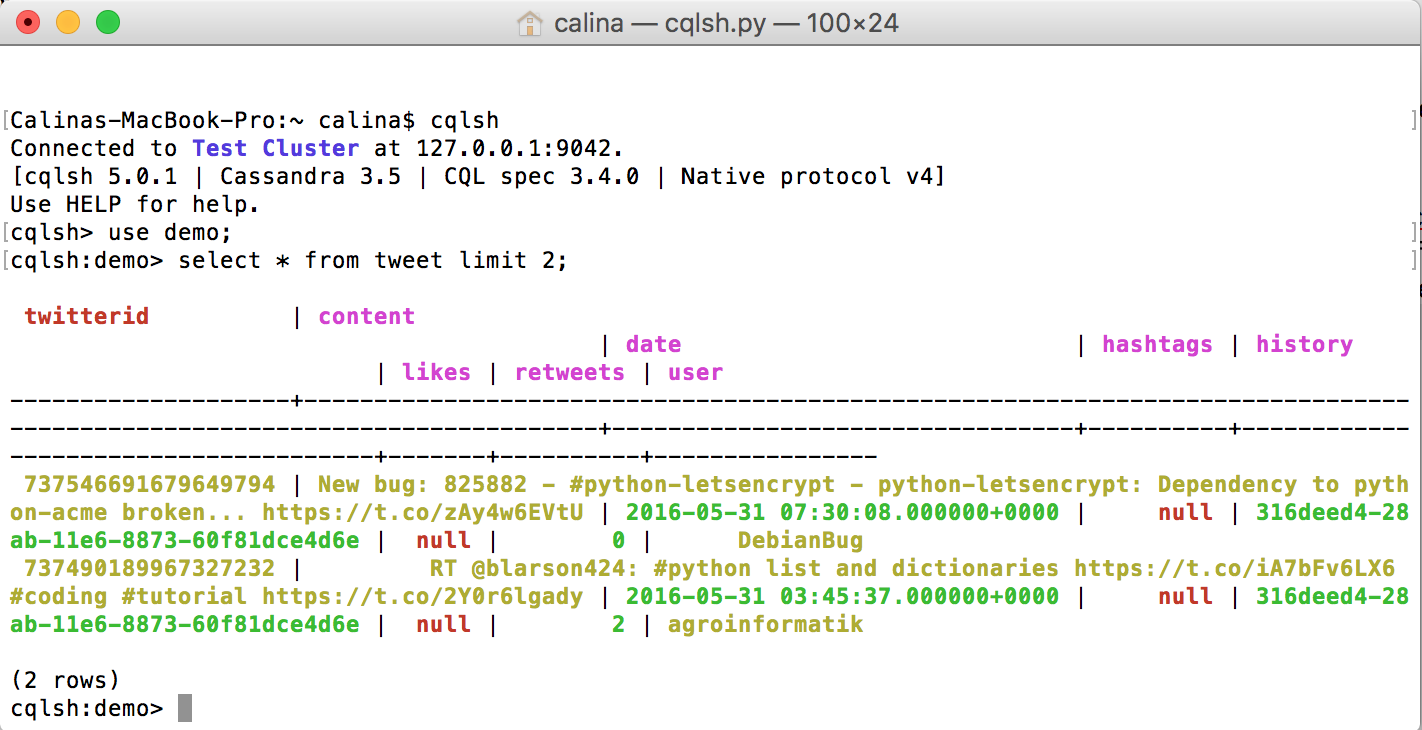
\includegraphics[width=0.8\columnwidth]{img/cqlsh.png}
    \caption{Demo of the cqlsh utility}
    \label{fig:cqlsh}
\end{figure}

The same functionality can be mirrored in Python using the following set of instructions:

\lstset{basicstyle=\scriptsize}
\begin{lstlisting}
from cassandra.cluster import Cluster

cluster = Cluster()
session = cluster.connect('demo')

 harvests = session.execute(
    """
    select * from tweets limit 2
    """
)
\end{lstlisting}

with the result being a generator which can be further consumed by the application. This means that it is easy to perform queries programatically, without much overhead, by employing the usage of this driver.

Cassandra queries are used throughout the application, both in synchronous and asynchronous application steps. Its speedy retrieval and updating of records is not a bottleneck, as API rate limits are.

\subsection{Database structure}
Two tables are used in our application. The \texttt{harvest} table containing columns:

\begin{itemize}
\item uuid (primary key, generated for each user-submitted harvest form)
\item start date (from which we harvest Tweets)
\item end date (up to which we harvest Tweets)
\item hashtag (used to query Twitter's API for statuses containing this particular hashtag)
\item done (boolean fag indicated whether the harvest has finished downloading Tweets)
\end{itemize}

The \texttt{tweet} table is used for storage of tweets belonging to histories and contains:

\begin{itemize}
\item twitterId (the id of that status on Twitter)
\item user (username of the author on Twitter)
\item content (textual content including hashtags)
\item date (of postage)
\item retweets (number of retweets, indicating popularity)
\item history (uuid of harvest that Tweet belongs to inside ATHENA)
\end{itemize}

\section{Harvesting tools}
The harvesting module as presented conceptually in \ref{fig:harvestpipe} was implemented in ATHENA using asynchronous job queueing. The user is presented with a form for submitting the harvesting job, consisting of a content field, start and end dates. An asynchronous job is launched via Python's Celery task library, which uses the tweepy library to connect to the Twitter Search API and Cassandra driver to save tweets and harvests.

\subsection{Celery for asynchronous jobs}
The Python library Celery\footnote{http://www.celeryproject.org} is designed for the fairly frequent development case where asynchronous jobs need to be managed. The Producer-Consumer architecture is implemented with Celery, as used in its real-time mode, while another option would be using Celery to run scheduled jobs. The job granularity in this case is indeed Harvest-level, with each job inside the Producer-Consumer queue is defined as the job of downloading one single, separate Harvest.

As previously stated, a huge advantage of Python is that third party libraries are highly compatible and easily configurable. Such is the case with Celery as well, setting up an asynchronous jobs taking very little effort:

\begin{enumerate}
\item install the \texttt{celery} library using \texttt{pip}
\item add configuration information to a celery.py file inside the application directory, including the task body and its decorator \texttt{@app.task(bind=True)}
\item import the function and use it. In the ATHENA Harvesting module context, the function was added as part of the Form validation customisation in Django's FormView class
\item install and configure a service broker such as Redis
\end{enumerate}

\subsection{Using Redis as a Celery broker}
Celery offers a variety of possible brokers for message transport through the job queue. Stable brokers are RabbitMQ and Redis, while others are in Experimental stages or offered by third parties\footnote{http://docs.celeryproject.org/en/latest/getting-started/brokers/}. Redis is an open source data structure store which can perform as a database or cache system, but in our case we are interested in its functionality as a message broker.

Installing Redis is straightforward using a downloaded package and even some available package managers such as Mac's \texttt{brew}. After the installation is complete, the Redis server can be fired up using the command \texttt{redis-server}. A splash screen with Redis' logo as ASCII art, such as the example in \ref{fig:redis} should appear, but connection to the running Redis server can also be tested by pinging:

\lstset{basicstyle=\small}
\begin{lstlisting}
$ redis-cli ping
PONG
\end{lstlisting}

\begin{figure}[ht]
    \centering
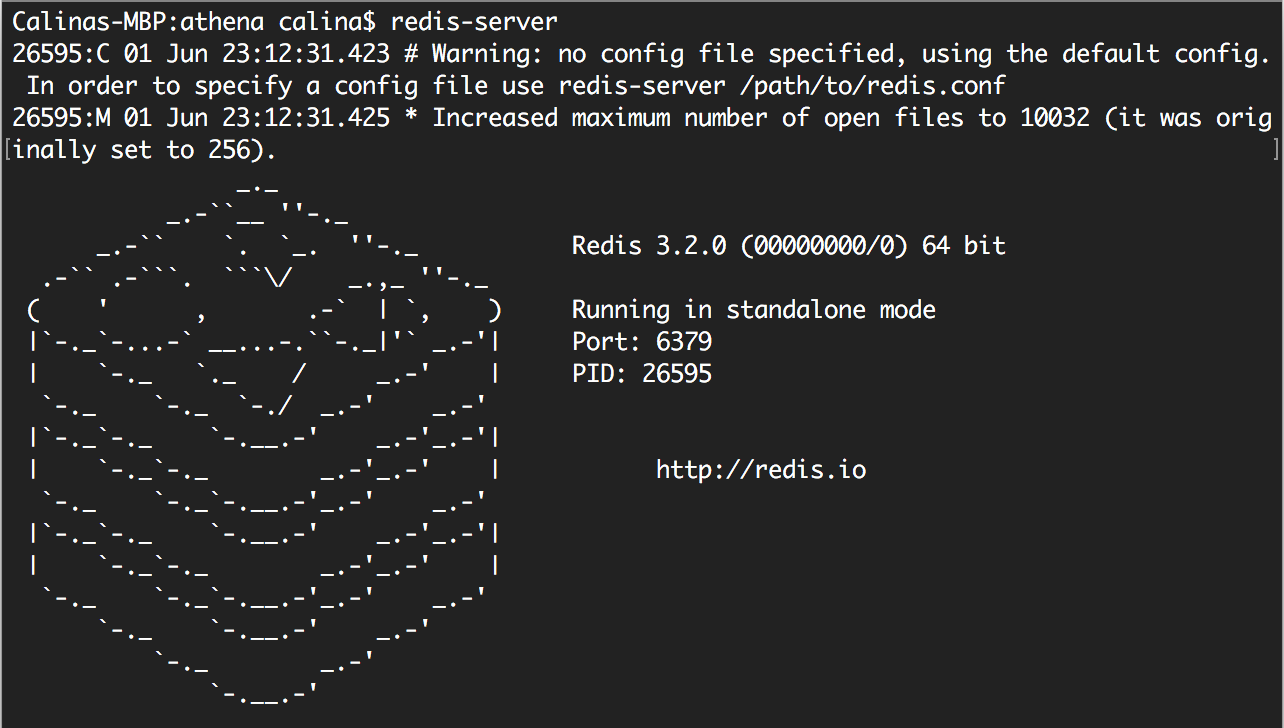
\includegraphics[width=0.8\columnwidth]{img/redis-splash.png}
    \caption{Redis splash screen}
    \label{fig:redis}
\end{figure}

After the Redis server is properly installed and running, there are some extra steps for hooking it up: adding the Redis configuration settings in our project's \texttt{settings.py} file and installing the \texttt{redis} library using pip. After all these steps are completed, running:

\lstset{basicstyle=\small}
\begin{lstlisting}
celery -A athena_app worker -l info
\end{lstlisting}

should confirm Celery's connection to Redis. Any tasks that were previously set up will now go through this job queue.

\subsection{Fetching data from Twitter using the Search API and Tweepy}
Once the general configuration of the asynchronous job is done, we can use the Twitter Search API to Harvest tweets per the specifications.

Twitter belongs to a series of web applications which fully understands the developers' need to hook into some of their features. Creating a Twitter application is easy from their developer support pages, with the creator receiving a set of OAuth access keys:

\begin{itemize}
\item a Consumer Key (API Key)
\item a Consumer Secret (API Secret)
\item an Access Token
\item an Access Token secret
\end{itemize}

For harvesting tweets, my approach uses a wrapper to Twitter's Search API called Tweepy\footnote{http://tweepy.readthedocs.io/en/v3.5.0/}. It is a library that handles connection and customised requests to the API, in a Pythonic fashion. Tweepy needs to be installed using pip, and then configured with the proper access keys (here in the code sample replaced with placeholders for security purposes):

\lstset{basicstyle=\small}
\begin{lstlisting}
from tweepy import OAuthHandler

consumer_key="XXXX"
consumer_secret="XXXXXXXX"

access_token="XXXX"
access_token_secret= "XXXXXXXX"

auth = OAuthHandler(consumer_key, consumer_secret)
auth.set_access_token(access_token, access_token_secret)
\end{lstlisting}

The way I am using this is by first setting up an \texttt{api} object which I will further query for statuses. I will initialise it using the \texttt{auth} object and a few flags:

\begin{itemize}
\item \texttt{wait\_on\_rate\_limit=True}. Flagging this indicates to the api object that whenever it reaches the API rate limits, it should not stop, but rather sleep for the required amount of time until new data can be acquired. This approach is preferable, since our harvesting takes place asynchronously and we do not mind the process sleeping for a while
\item \texttt{wait\_on\_rate\_limit\_notify=True}. Setting this flag tells the api object to print out a warning string to the console, indicating when it has reached the rate limit and at the beginning and end of the sleep cycle. E.g.:\lstset{basicstyle=\small}
\begin{lstlisting}
[2016-06-02 10:17:46,804: WARNING/Worker-2]
Rate limit reached. Sleeping for:
627
\end{lstlisting}
\end{itemize}

After setting up the API, a Tweepy Cursor class is used for querying it. This is initialised with the api object and parameters indicating the query we send to the server. This uses parameters defined by the user upon submitting the harvest form, refined by our application's specifications. The hashtag field is prefixed with a "\#" sign, start and end dates are formatted to "yyyy-mm-dd" and the language set to English, since extension to other languages is beyond the scope of this thesis.

The cursor will return a Pyhton generator, which means that the contents of the tweet list is rather consumed one by one, rather than having the whole list present at either point in time. Here, using Cassandra, we save the contents to the database.

\lstset{basicstyle=\small, breaklines=True}
\begin{lstlisting}
tweets = tweepy.Cursor(api.search, q='#' + hashtag, since=start_date, until=end_date, lang='en').items()

for tweet in tweets:
    session.execute(
     """
     insert into tweet (twitterId, user, content, date, retweets, history) values (%s, %s, %s, %s, %s, %s)
     """,
     (str(tweet.id), tweet.author.screen_name.encode('utf8'), tweet.text, tweet.created_at, tweet.retweet_count, key)
     )
\end{lstlisting}

The stored and completed harvests are now ready for the Enhancement step.

\section{Enhancement tools}
Enhancement tools are concentrated in the enhancement\_manager.py file/module where basic numerical calculations on the data is performed, alongside more complex transformations such as related hashtag collection and hashtag clustering. The process of enhancing data starts on the Enhancement tab, with the user being presented the list of available Harvests. The user decides on the harvest they want to enhance and display by clicking an icon next to the harvest's title.

\subsection{Simple numerical data}
A number of easily calculated, relevant data is calculated for the user and displayed on the enhancement results page. The number of tweets is calculated using a database query and displayed in a separate \texttt{<div>} on the results page.

\subsubsection{User-related data}
Upon consuming the tweet generator which resulted from the query, the data related to users is restructured as a Pyhton dictionary having the usernames of keys and the number of documents authored by those users, in the contex of the present harvest. The following numerical data is displayed related to users:

\begin{itemize}
\item the number of unique users contributing tweets to the enhanced harvest
\item the maximum number of tweets per user. The author's username is also presented in parantheses, and will usually represent a bot or a domain-related page, e.g. for the \texttt{\#pyhton} hashtag, the highest number of posts in a given day is posted by the user \texttt{@pyhtonbot\_}
\item the average number of posts per user, which is a metric indicating the general activity level of the harvest's generator hashtag
\end{itemize}

\subsubsection{Modeling the post numbers}
Since many a times the number of posts per user tends to skew towards pages and bots, it may be the case that the number of posts indicate a certain pattern. To analyse the eventuality of post numbers as an estimation of a power function, the \texttt{plfit} library was used. First the data was prepared as a list, from the users/posts dictionary described above. 

The \texttt{plfit} library was originally written in Matlab by Clauset et al \cite{clauset2009power} and later converted to R, Python and C++ modules by various developers. It handles calculations regarding data pattern fitting to a power law as described in \ref{plfittheory}. The library is suitable for non-domain-related data, being based on a combined maximum-likelihood fitting and goodness-of-fit tests. It was tested on twenty-four real-world data sets from unrelated fields of study and has found good results with power law fitting.

After importing the \texttt{plfit} library into the enhancement module, a plfit object is created. The tweet numbers are then fitted using the plfit method on the list described above. The minimum value and alpha are printed on the enhancement results page.

\subsection{Sci-kit learn}
Sci-kit Learn\footnote{http://scikit-learn.org/stable/} is proof of the fact that Python has recently gained much momentum in science and research. Its architecture is build on other stable and related Python science libraries, namely NumPy, SciPy and matplotlib. In fact, upon installation with the \texttt{pip} command line utility, sci-kit also installs these libraries as dependencies. According to a large number of scientists \cite{pedregosa2011scikit} and as displayed on their website, sci-kit learn is used for supervised and unsupervised data mining and data analysis endeavours, including:

\begin{itemize}
\item Classification
\item Regression
\item Clustering
\item Dimensionality reduction
\item Model selection
\item Preprocessing
\end{itemize}

Other important advantage of this library is its open souce BSD licensing. This means that, even tough it is a highly specialised tool, it is free to use for developers worldwide. The following presents \emph{sci-kit learn}'s employment in ATHENA.

\subsection{Related hashtag calculation}
Twitter uses a hashtag system to encourage users to tag data for proper search and visibility. Hashtags are words prefixed by a "\#" character, which represent categories of statuses. The hashtag system has been used on Twitter ever since its start, as opposed to other social networks such as Facebook, who only employed tagging much after being launched. Such other social networks have a hashtag disadvantage, since the system did not "catch on" with their users as naturally as it has on early-adopters such as Twitter.

On going into the realm of more complexly calculated data, as opposed to the numerical values extracted directly from the list of tweets, calculating a harvest's related hashtags is a more difficult task and is achieved using sci-kit learn. Figure \ref{fig:tweet} presents a sample tweet (the screenshot was taken on 7th June 2016), and it is clear empirically from such status messages that hashtags can be interpreted as category labels.

\begin{figure}[ht]
    \centering

\includegraphics[width=0.8\columnwidth]{img/tweet.png}
    \caption{Sample status message with hashtags}
    \label{fig:tweet}
\end{figure}

The tweet in Figure \ref{fig:tweet} also empirically demonstrates that the same post belongs to a number of related categories, in this case \emph{yoga}, \emph{fitness}, \emph{lolesport}, \emph{gym}, \emph{cardiotime}, \emph{sports}, \emph{workout} and \emph{zumba}. Indded these hashtags seem much related to one another, in this case, all belonging to a domain of sport and fitness.

Analysing each status' component hashtags will reveal related hashtags. As part of the enhancement process, we consider all the related collected tweets which compose a harvest and go trough the \texttt{get\_vocabulary} function, much like in the grammatical process of collecting a word's semantic field.

\subsubsection{Getting the hashtag vocabulary}
For the purpose of getting the list of related hashtags to our own harvest's base hashtag, we use a few customised components from the \emph{sci-kit learn} toolbelt. I start by vectorizing the list of tweets using the \texttt{TfidfVectorizer} with the following options:

\begin{itemize}
\item \texttt{min\_df=10}, to prevent hashtags who appear in less than 10 tweets appearing in our final list of results. This prevents noise generated by use-once hashtags through unusual, parody or disparate hashtags.
\item \texttt{max\_df=0.8}, to prevent flooding with most-common hashtags appearing in more than 80\% of the corpus
\item \texttt{sublinear\_tf=True} to use a sublinear function. A linear idf function may boost the document scores sometimes, but since the frequency of a term to relevance is usually a sublinear function, we use this option to ensure higher-precision results.
\item \texttt{use\_idf=True} to enable inverse-document-frequency re-weighting
\item \texttt{max\_features=25} to limit our search of most relevant related hashtags to a number of 25. We do this so that only the best most relevant hashtags are displayed for the user and prevent them being distracted by too much information.
\item \texttt{token\_pattern='\#[a-zA-Z0-9][a-zA-Z0-9]*'}. This option takes a regular expression (RegEx) argument which it uses to identify relevant tokens inside the corpus. Since we are only interested in hashtags and not other content words, the RegExp introduced forces the vectorizer to only consider "words" that start with a "\#' symbol and has one or more alphanumerical characters afterwards.
\end{itemize}

The sparse matrix indicating term frequency is obtained using the initialized vectorizer to \texttt{fit\_transform} the list of tweets' texts. Although a sparse matrix would overwhelm a non-expert user, and I have chosen not to display it as part of the enhancement results, the structure's content can be printed on the console and used for debugging and bird's eye correctness checking.

\begin{figure}[ht]
    \centering
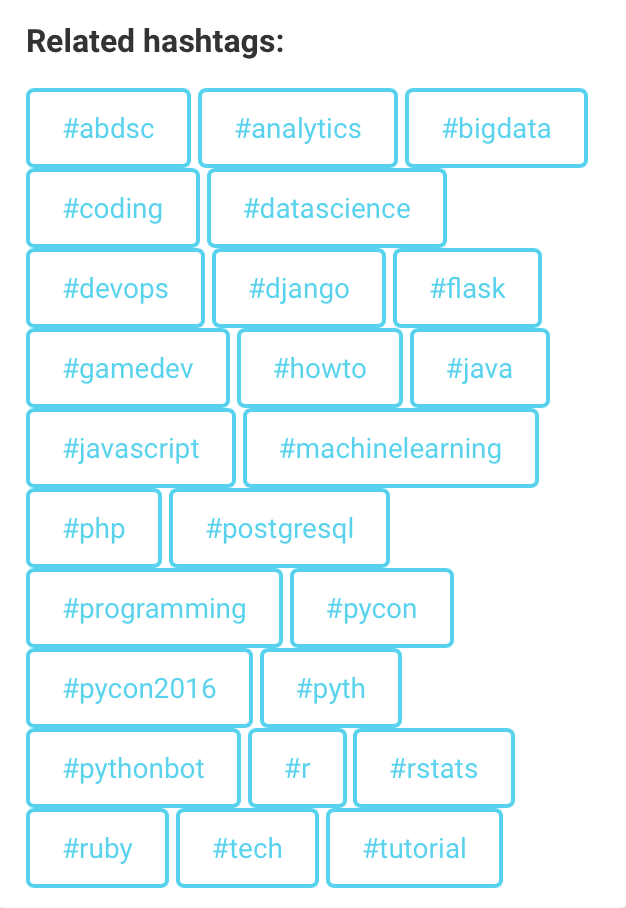
\includegraphics[width=0.4\columnwidth]{img/relhashtags.png}
    \caption{Example of related hashtags in a \#Python harvest over one day}
    \label{fig:relhashtags}
\end{figure}

We do however return the \texttt{vocabulary} variable. We calculate this by having the vectorizer perform the \texttt{get\_feature\_names()} method. This enables us to print a list of related hashtags on the enhancement results page in a separate \texttt{div}, as exemplified in Figure \ref{fig:relhashtags}. Indeed the empyrical data obtained in the example for the \#python hashtags showcases some of Python's most popular features (\#bigdata, \#machinelearning), tools (\#django, \#flask) and related technologies (\#javascript, \#ruby, \#r).

\subsection{Related hashtag clustering using KMeans}
Another interesting aspect the hashtags indicate is that there are some general directions (or common features) of our text. In a supervised approach, this could be tackled with an adnotated training dataset which would help classify the data. However, since ATHENA is based on user input and analysis of non-domain-related documents, such an approach is not appropriate.

One of the most classic approaches in classifying non-adnotated data is the K-Means clustering algorithm. Luckily \emph{Sci-kit learn} also contains tools for clustering approaches, including various implementations of K-Means variants.

Calculations start similarly to the approach described above, for related hashtags, but features an extra step for clustering. The concern for choosing a number of cluster centroids was similar to the one choosing the number of related hashtags to be displayed: A number of 5 centroids was chosen with the goal of having enough diversification, but not too many clusters to display, so as not to confuse the user. In a more domain-tweaked approach, the number of clusters would have been chosen according to the data's structure, but here it is a trade-off between the various factors explained.

A new \texttt{TfifVectorizer} object is instantiated with similar options, except for the \texttt{max\_df}, in order to also consider highly-used hashtags. After reproducing the \texttt{fit\_transform} step and obtraining the fitted set X, we apply the KMeans algorithm as such:

\lstset{basicstyle=\small, breaklines=True}
\begin{lstlisting}
from sklearn.cluster import KMeans
[...]

model = KMeans(n_clusters=true_k, init='k-means++', max_iter=100, n_init=1)
model.fit(X)
\end{lstlisting}

For the centroid initialisation, I chose the "K-Means++" algorithm described in \ref{kmeansplusplus}, a maximum number of iterations towards the solution of 100. The \texttt{n\_init} option instructs the K-Means algorithm to run  just once with different centroid seeds. In case a larger number would have been chosen, the output of the algorithm would have been the best output during these runs.

\subsubsection{Ordering and displaying the hashtag clusters}
The main issue with clustering generation, as directly resulted from the \emph{Sci-kit} K-Means algorithm, is that the clusters are not ordered. Items are assigned with some probability to each cluster, but there is no clear representation and collection of those clusters. In order to properly display these clusters on the results page, though, they need to be sorted and formatted.

\lstset{basicstyle=\small, breaklines=True}
\begin{lstlisting}
order_centroids = model.cluster_centers_.argsort()[:, ::-1]
terms = vectorizer.get_feature_names()
clusters = {}

for i in range(true_k):
    cluster_name = 'Cluster ' + str(i+1) + ':'
    cluster = {}
    for ind in order_centroids[i, :10]:
        cluster[ind] = str(terms[ind])
    clusters[cluster_name] = cluster

    return clusters
\end{lstlisting}

Note the similarity to the previously described feature. The terms are fetched just the same, and then their assignment to the clusters is checked. The resulting structure is a dictionary consisting of cluster names as keys and hashtags (from the same cluster) as values.

They are returned to the controller, then to the front-end part and displayed via Django's templating engine. For a better understanding of their separation, each cluster is placed into its own div with Bootstrap's \texttt{well} CSS class, which adds a separate wrapper and colouring to its contents. Figure \ref{fig:clusters} presents an example of such a clustering.

\begin{figure}[ht]
    \centering
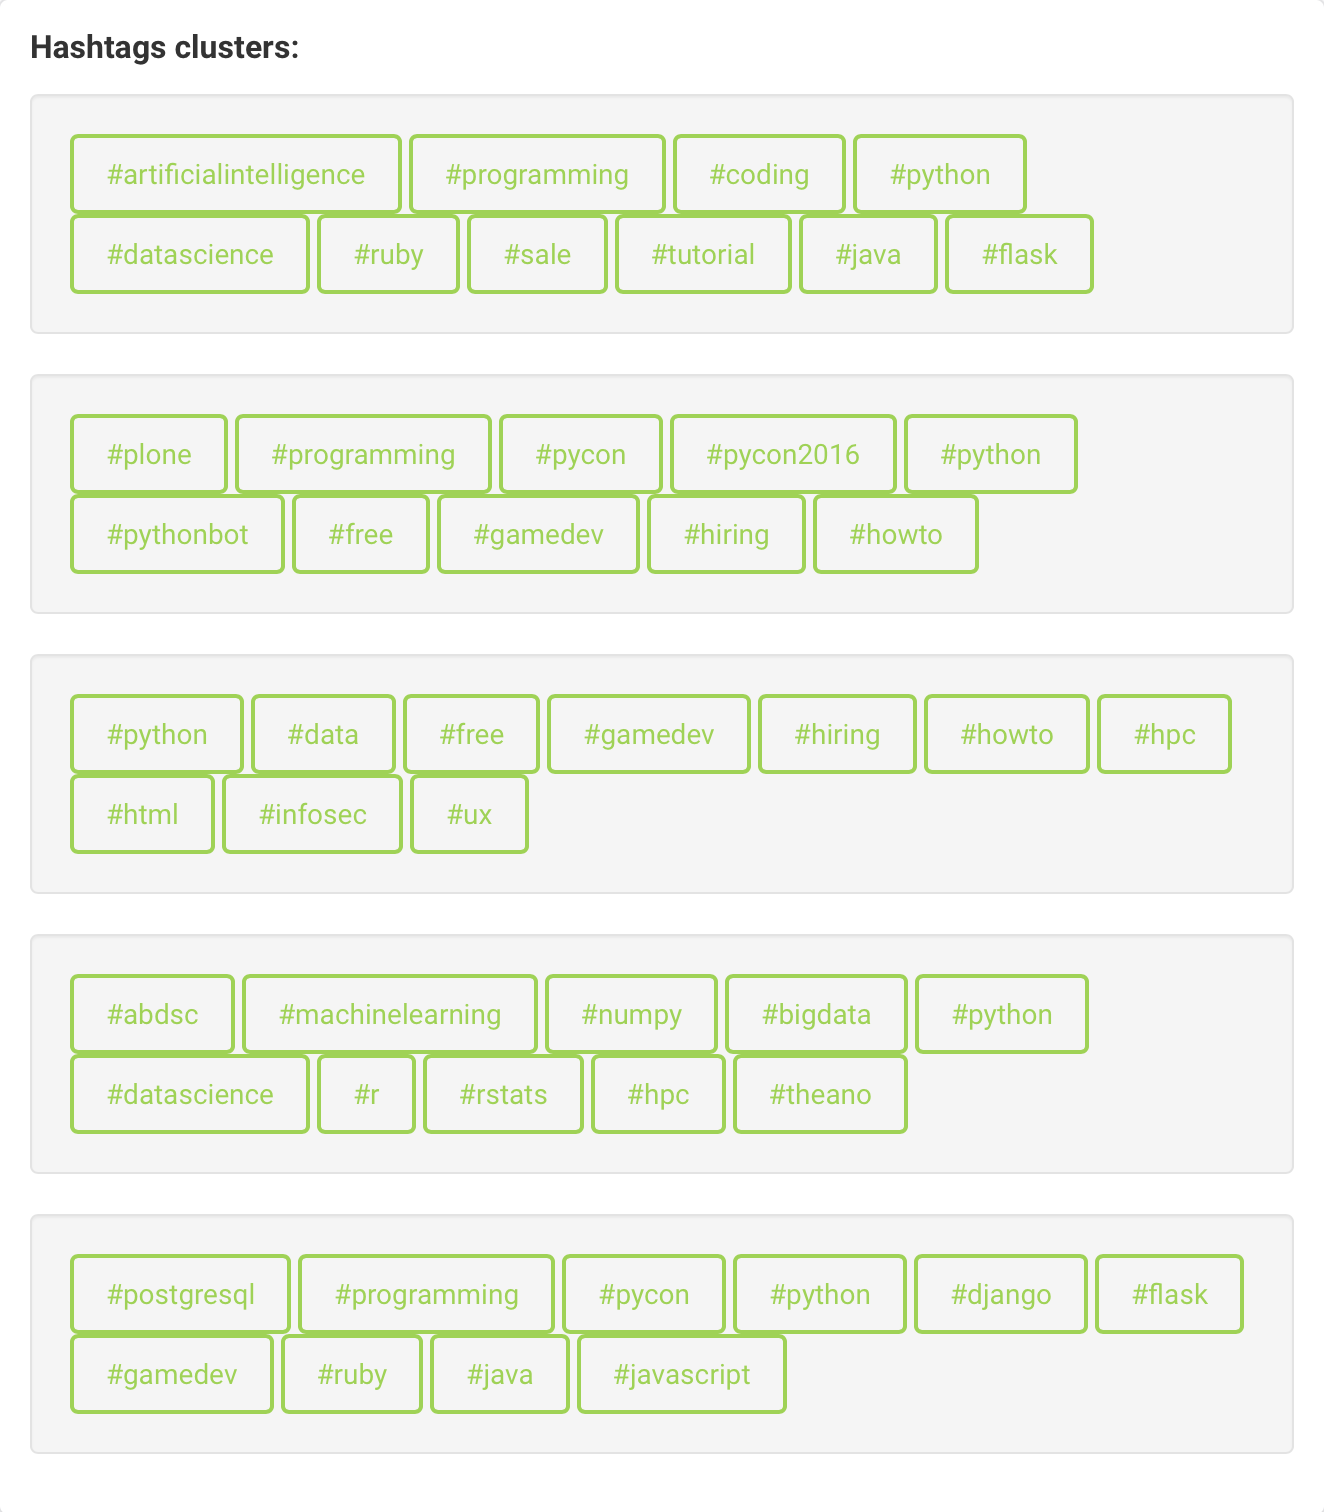
\includegraphics[width=0.7\columnwidth]{img/clusters.png}
    \caption{Example of clustered hashtags in a \#Python harvest over one day}
    \label{fig:clusters}
\end{figure}

It can be seen in the example that the clusters follow a structure similar to Python's main fields of development.

\begin{enumerate}
\item the first cluster is correspondent to some genric Python fields: \#flask, \#coding, \#artificialintelligence
\item the second cluster is correspondent to Python conventions, promotions and opportunities for development: \#free, \#gamedev, \#hiring, \#pycon
\item the third cluster relates to front-end technologies and their prevalence in Python conventions: \#html, \#ux
\item the fourth cluster relates to Python's endeavours in machine learning: \#machinelearning, \#bigdata, \#numpy, \#datascience, \#r, \#rstats
\item the fifth cluster is a collection of technologies related to Python or generally used alognside it: \#postgresql, \#django, \#flask, \#javascript
\end{enumerate}

New clustering is calculated with every refresh, and the user can observe a high degree of convergence for rich hashtags such as our \#python example. For one-fold or loosely related hashtags, the number of centroids chosen might indeed be too large.

\section{Normalisation}
\subsection{Reasons and options}
As previously discussed, many a times the dataset is skewed due to spikes and outliers such as pages and bots. The normalisation step helps with the process of eliminating outliers and possible fakers, by flattening the dataset to a single representative post per each user. This is done mostly because professional pages intentionally use repetitive hashtags to promote certain events. On the other hand, bots scan for and retweet statuses which feature specific content, which results in the flooding of the dataset with promotional messages. Both these series of events lead to skewed dataset wich is easily recognisable by its fitting to a power function.

Remember that the Enhancement step only takes regular harvests as inputs, as it calculates power set fitting, likely pages and outliers etc. In a similar fashion, the Analysis step will only consider normalised harvests as permitted input. This means that output of the Normalisation step should be properly stored, in a separate table.

It must also be noted that the Normalisation step is still in its early proof of concept ages, since the main focus of this application was to develop and validate the Harvesting, Enhancement and Analysis steps, and only then add more functionality to the Normalisation module. Proper Normalisation should indeed take into consideration various factors:

\begin{itemize}
\item flattening process: 
\begin{itemize}
\item one post per user, to remove outliers such as pages and bots
\item multiple posts-only, to analyse only regular users, which use the hashtag more times, which would filter out accidental ones with opinions that might be unrepresentative for the community
\item popular posts-only, considering only posts with retweet count larger than a threshold $r$
\item liked posts-only, considering only posts with like count larger than a threshold $l$.
\item combinations of the above options
\end{itemize}
\item time period considered
\begin{itemize}
\item short term options: $n$-days with $n\leq7$, $m$-hour normalisation
\item long term options: $n$-days with $n>7$, which would also imply the possibility of streaming harvests on a longer period, per Twitter API's rate limits.
\end{itemize} 
\end{itemize}

Each normalisation method has its very own advantages and drawbacks, so in order to choose a viable normalisation method to implement, the following was considered: Unfortunately with promotional messages such as those posted by pages and bots, the retweet and like counts is often tied to some form of prize or gratification a user gets for sharing the content. This means that the popularity of the tweet is many a times artificially boasted using a variety of marketing methods. Also, it might be the case that few users actually post multiple tweets in a short-term amount of time, which rules out the second option of flattening as well.

Current implementation restricts normalisation options to one post per user and one-day date limits. However, the code is designed in such a fashion that new options should be added easily, when the need arises.

\subsection{One post per user, one-day limit normalisation process}
The process I describe below is currently the only allowed Normalisation process, with more to come after testing and user validation of the ATHENA proof of concept app. This method of normalisation intends to remove outlier influence of pages, bots and fake accounts.

The first interface presented to the user in the Normalisation step is a form containing the list of harvests in a dropdown. After submitting the form, the selected harvest is sent to the \texttt{normalisation\_manager.py} file through the controller. This manager file contains the process necessary to fetch the harvest's tweets from the database and flattening the result into a list.

The method used was the classical approach of duplicate removal using HashMaps (as implemented in the Python dictionary data type). Using the username as the dictionary's key, the last occurrence in the list of tweets for each user is considered. The value of this result dictionary is a tuple of tweet id and tweet content, which are later used in the Analysis module. Of course, the tweet's post date is also considered, in order to filter out tweets outside the date limit.

Results are stored in the \texttt{normal} database table, which has a structure consisting of the following columns:
\begin{itemize}
\item original harvest uuid, which facilitates comparison between corresponding normalised and regular harvests
\item name of the normalised harvest (formed using the original harvest's name and the normalisation type details)
\item JSON-serialised normalised dictionary resulting from the normalisation step
\end{itemize}

Or, as CQL script:
\begin{lstlisting}
CREATE TABLE normal (uuid uuid, name text, content text, PRIMARY KEY(uuid));
\end{lstlisting}

Multiple formats would have been suitable for serialisation if persistence only was considered. But in the idea of adding a RESTful module to the application, enabling its use from mobile and web applications seamlessly, the normalisation result is stored in a JSON format. JSON is a widely-spread and widely-used format for REST service communication and is easily integrated with Python and Django via the \texttt{json} library. The contents of the Python data structure is encoded using \texttt{json.dumps()}, while the loading from a string and into a Python data structure can be achieved using \texttt{json.loads()}.

\section{Analysis}
The Analysis module features a lot of similarity to both Enhancement and Normalisation, except that in both cases, the pages contain double the harvests. Firstly, the form step of Analysis contains two dropdowns which are populated with normalised harvests. After choosing a pair of harvests for comparison, the application redirects to a page displaying the analysis results.

As per previous modules, this one also has a dedicated manager file, called \texttt{analysis\_manager}. Analysis jobs are therefore passed from the controller to the manager and the results are sent back after calculation. A number of analysis types are run on the normalised harvests, including common vocabulary, common users and post proportions.

\subsection{Retrieving the normalised results}
The task of retrieving the previously saved normalised results is a fairly simple one, consisting of connecting to the database, running a query to select the two normalised entries as selected in the form (using their respective uuids) and deserialising the JSON string in the content using the \texttt{json.loads()} function. The deserialised result is exactly as the one calculated in the Normalisation step, i.e. the keys are the users and the values are tuples of significant data, including tweet content.

\subsection{Calculating the common vocabulary}
The common vocabulary of hashtags is a type of analysis inspired from the previous Enhancement step. We are interested, in case of hashtag pairs belonging to the same fields or domains, in their very own, particular characteristics (handled here with Enhancement), but also in some common values which the share. One such important question is whether there are any common labels between the two.

Common vocabulary generation is very much similar to vocabulary generation, as done in the Enhancement module. Hence the calculation consists of both respective vocabularies intersected. This means that the vocabulary function from enhancement can be reused in a DRY (Do not Repeat Yourself) fashion. The operation of intersection is done using the \& operator between the two sets, which is an efficient way of getting the result without much code written.

Figure \ref{fig:commonvocab} shows an example of results for the comparison between one-day normalisations of the \#python and \#php hashtags, indicating two general categories the two belong to (\#programming and \#coding), and two technologies usually associated to them, one on the front-end side (\#javascript) and one on back-end (\#java)

\begin{figure}
    \centering

\includegraphics[width=0.5\columnwidth]{img/commonvocab.png}
    \caption{Example of common vocabulary in \#Python vs \#PHP comparison}
    \label{fig:commonvocab}
\end{figure}

\subsection{Calculating common users}
Common users are calculated in a similar fashion to that described above. Since the result deserialised from the database is a dictionary with unique keys (Python dictionaries are based on an underlying HashMap structure), the only task is to combine the two key arrays using an intersection operator, as previously done for the vocabulary part, e.g.:

\[common\_users = set(h1\_users) \& set(h2\_users)\]

\subsection{Calculating post numbers and proportions}
Another important metric is the prevalence of posts belonging to a harvest as part of the domain. In comparing two normalised harvests, we are interested in the proportion of each exclusive tag and also the number of common posts. These metrics show whether one or the other hashtag is the most productive in number of posts, which may indicate number of supporters. Furthermore, by analysing the numbers and proportions of these posts, we can deduce whether the domain is clearly split between the two hashtags, or whether there is a lot of gray area, which contains posts belonging to both categories. This latter option would indicate that supporters of both concepts are fluid and have no clear preference, while a clear separation could indicate die-hard fans.

Of course this relation can be exploited in a number of ways. In a very hostile, polarised domain, the user can analyse the risks of appealing to one of the groups, while rejecting the other. However in a cohesive domain with much middle ground, a good option is to appeal to the general unifying concepts.

In order to calculate the domain breakdown between the two normalised harvests, we consider users as a point of reference. We have already calculated the set of common users during the previous steps, so now we calculate the difference sets using the lists of posting users in each harvest and excluding the common ones.

Of course displaying the raw numbers on the results page doesn't help the user that much. It is therefore necessary to perform some extra steps to indicate the polarisation of the domain between the two hashtags: displaying the numbers as a graphical pie chart. Such a chart indicates the proportions of users who post exclusively for each hashtag and common users, who represent the middle ground.

Figure \ref{fig:piechart} presents the results for the user proportions between two hashtags: \#python and \#php. The results indeed seem to match with empyrical real-life data, since the two are both back-end programming languages and it is rarely seen that both are used by the same people or in the same projects. Results also display a highly-polarised domain, with a slight better cult of Python, which can be confirmed from other sources such as the TIOBE index, which maintains Python is more popular than PHP.

\subsubsection{Displaying the chart using Google Charts API}
A number of approaches for HTML charting are available for free use. Some work primarily on the back-end with image generation, while some are exclusively front-end. Among the simplest and easiest to use approaches is using Google Chart API, a javascript library for front-end chart generation. The image in \ref{fig:piechart} is captured from the application and is indeed generated using Google Chart API. The code is fairly straightforward, using javascript on the front-end side, from the list of values.

\begin{lstlisting}
var data = google.visualization.arrayToDataTable([
      ['Norm. Harvest', 'Number of posts'],
      ["{{ h1 }}",     {{ proportions.0 }}],
      ["{{ h2 }}",     {{ proportions.1 }}],
      ["common",     {{ proportions.2 }}],
    ]);
\end{lstlisting}

Note that the curly brackets used are from Django's templating engine, and are variables which are passed from the controller onto the view. When executing the javascript code, the values are already replaced with the corresponding values and will execute like normal strings or numbers within the code.

Hovering the mouse over one pie chart slice generates a dialog containing both the raw number and the proportion from the total, as shown in the figure as well, onto \emph{php one day normalisation}.

\begin{figure}
    \centering
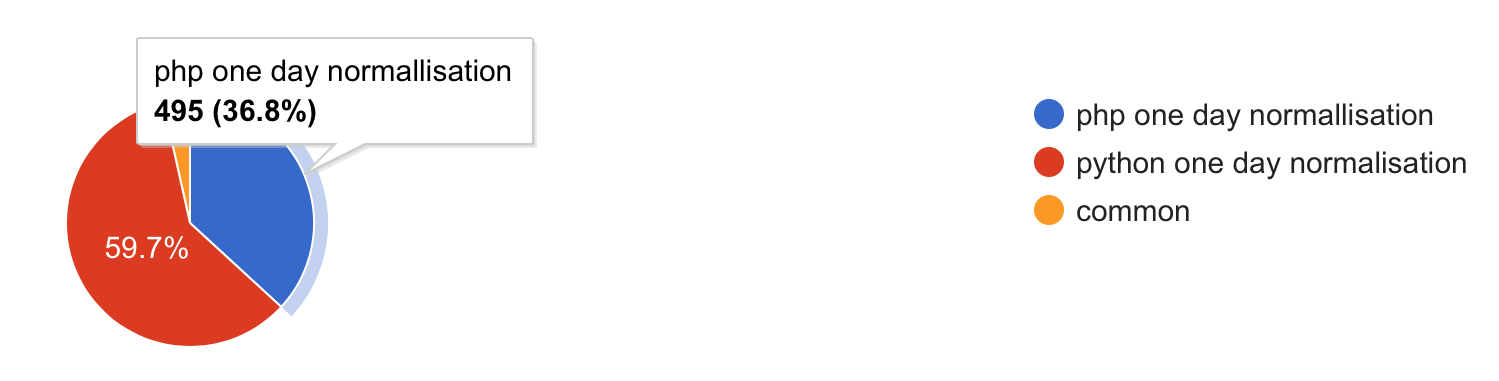
\includegraphics[width=\columnwidth]{img/piechart.png}
    \caption{Proportions of users who post \#Python vs \#PHP tagged statuses}
    \label{fig:piechart}
\end{figure}

\section{Code organisation}
Generally speaking, the code is organised in a classical MVC (Model-View-Controller) fashion, with specifics related to Django's recommentations. As per their recommended usage, the functionality is separated into an app called \texttt{athena\_app} found in the \texttt{athena} workspace, under a virtual environment wrapper with Django 1.8 installed. 

\subsection{File and folder structure}
As Django tends to encourage reusability, some of the scaffolding and file structure is generated via commands using the \texttt{manage.py} command line utility. E.g., upon creating a new app, a directory structure is also created containing:

\begin{itemize}
\item \texttt{urls.py}, the file which contains URL path definitions and directs received data to the corresponding views, as defined by the user. Our application currently defines a total of 8 URLs, for the index page, harvest, enhancement, normalisation and analysis page as well as some result pages. The local \texttt{urls.py} file is imported into the main \texttt{urls.py} which resides in the root of the project.
\item \texttt{views.py}, the file which contains what other frameworks call "controller actions". These functions determine the behaviour of the application when encountering the data matched by respective entries in \texttt{urls.py}. As a general best practice, our functions in \texttt{views.py} either inherit and override significant parts of Django generic views\footnote{Code templates for widely-used functionalites such as CRUD, forms or simple HTML rendering views}, or use minimal code and delegate to manager files for the core functionality.
\item \texttt{models.py}, which should contain model definition. This file was not used, since database queries were written manually in CQL, which is not that well supported by Django's migration creating structure for models and migrations.
\item \texttt{forms.py} which contains form definitions, holding part of the functionality, field definitions and validation instructions
\item other various folders such as the \texttt{static} folder where static files such as images, CSS and JS are stored, and the \texttt{templates} folder where html views are stored. Our application's static folder contains various Twitter Bootstrap CSS and JS elements for beautifying the front-end, while our templates directory holds a number of 6 individual views (mostly corresponding to the URLs enumerated above) and one \texttt{base.html} view which the others use as a general template. This enables us to only overwrite those sections which change and leave the menu and headers generally intact.
\item some other files and folders which we have not used and are beyond the scope of our application, such as \texttt{admin.py} (which should define administrative actions with Django Admin) and others.
\end{itemize}

Python's import structure is defined using file names and classes/functions defined inside those files. This makes it easy to use functions from files such as managers, by simply importing those functions. The separation of concerns principle is very important for proper maintenance and good functionality of the code, so the controllers stay light and handle Request processing and Response sending, while the core work is done separately in managers. The application defines a number of four managers:

\begin{itemize}
\item \texttt{harvest\_manager.py}, dealing with harvesting jobs and used primarily from the harvest parts of the \texttt{view.py} file
\item \texttt{enhancement\_manager.py}, dealing with the enhancement-concerned parts of the application
\item \texttt{normalisation\_manager.py}, dealing with flattening the datasets as instructed by the corresponding actions in \texttt{views.py}
\item \texttt{analysis\_manager.py}, containing analysis functions and used by the Analysis module
\end{itemize}

As previously stated, Python's simple structure make it easy to import functions from the managers inside the views using specific commands and then straightforwardly using the function, e.g.:

\begin{lstlisting}
from athena_app.harvest_manager import get_harvests
[...]
result = get_harvests()
\end{lstlisting}

\subsection{Using Django generic views}
Django offers the possibility of reusing specific classes from their very own codebase, classes which were designed for repetitive tasks. As opposed to having programmers code their very own implementations of rendering simple HTML views, creating and validation forms or performing CRUD (Create, Update, Delete) funcionalities, these classes, called generic views, can be directly used, or efficiently customised by overwriting a few attributes or methods.

ATHENA uses Django's \texttt{FormView} and the basic \texttt{View}, imported from

\texttt{django.views.generic.edit} and 

\texttt{django.views.generic.base}

respectively. The former is used for creating the Enhancement and Normalisation harvest selection page, and the Analysis pairwise normalised harvest selection page. FormView is also used when creating the harvest and is perhaps the most representative example, combining fields of various types and a special success method performed on return.

The HarvestForm is defined in \texttt{forms.py} and used inside the FormView in \texttt{views.py}. Inside the class definition an extra method was added, called \texttt{create\_harvest}, which is not an override of any parent method, but instead contains instructions on performing the asynchronous job of creating the harvest. Otherwise, the rest of the Form definition consists of field declarations with their corresponding types:

\begin{itemize}
\item \texttt{hashtag} as type \texttt{CharField}, the hashtag used for searching tweets on Twitter API
\item \texttt{start\_date} as type \texttt{DateField}, the beginning date for filtering tweets
\item \texttt{end\_date} similarly, represents the end date for tweet filtering
\end{itemize}

HarvestView inherits from Django's FormView and overwrites some fields and methods, which are somewhat instructive for understanding the other customised Forms and FormViews defined inside the application's codebase:

\begin{itemize}
\item template name: path of the HTML template to render
\item form class: the HarvestForm we defined in \texttt{forms.py} and imported here
\item success url: where the view should redirect upon form submission and success
\item get context data(): defines extra variables to be passed to the templating engine. In our case, it is the list of available harvests.
\item form valid(): extra validation and/or steps to be performed in case of success
\end{itemize}

In regards of the classic \texttt{View} generic, its only overwritten method was \texttt{get()} which instructs the view on the course it should consider when receiving a GET-type HTML request.

\subsection{List comprehensions and other Python specifics}
\label{listcomprehensions}
Python is a language of simplicity, but it is also a language difficult to understand from the outside. Its focus on simplicity starts from the building blocks: no visibility modifiers, easy import management, indentation-based execution blocks. However, some simplifications may seem obscure.

One of such shorthand becoming cipher is the declaration of arrays and lists, as in:
\begin{lstlisting}
    tweet_texts = []
    tweet_users = {}
\end{lstlisting}

This snippet first declares an array called tweet\_texts, while the second, tweet\_users, is a dictionary. To complicate things even worse, tuples are declared using round braces. This is in opposition to the generally verbose approach of other programming languages and is important to note.

On a related note, list and dictionary comprehensions are an efficient way of creating or filtering a list or dictionary with as less code written as possible. Code such as:

\begin{lstlisting}
[ ( x.uuid, x.name) for x in all_harvests ]
\end{lstlisting}

may be perceived as ambiguous for unfamiliar users. However for Python developers it becomes clear that this snippet produces a list of tuples from the iterable \texttt{all\_harvests}, with tuples containing the iterable element's uuid and name. In English, what this does it that it filters out some unnecessary properties in all harvests and transforms the list of objects into a simple list of pairs(uuid, name).

\subsection*{Summary}
In this section the details of implementation inside ATHENA were explained. The choice of Python and Django as programming language and frameowrk respectively were motivated by their large-scale use in developing scientific applications and web applications in general. The list of third party libraries was covered, with focus on particular libraries and their usage throughout the application.

The persistence model was chosen to be non-relational and scalable, in order to support scaling the system to a larger number of nodes and eventually moving towards a distributed web application. The task of fetching Twitter statuses was handled using asynchronous job running, using the Producer-Consumer architecture, via the Celery library with Redis as a message broker. This approach ensures the user doesn't have to wait for a job to finish before continuing to use the application independently. Inside the job, rate limits and concrete Twitter API communication were handled using Tweepy, a Python wrapper. The resulting, grouped information is called a Harvest.

The Enhancement step displays numerical data, a harvest's related hashtags and uses the acclaimed Sci-kit library to perform clustering on domain hashtags, using the K-Means algorithm. Another issue ATHENA tackles is the fitting of the post numbers dataset to a power function, investigating on outliers such as pages, bots and fake accounts producing significally more content than regular users.

The Normalisation step flattens the data set in a "one post per user, one day" fashion, with other normalisation options currently in development. The Analysis step uses the data flattened, filtered and stored by Normalisation to run a comparison between two harvests. Such data includes vocabulary commonalities and polarisation analysis.

The final part of this section approaches Python particularities which are used in the application but might seem unfamiliar to developers coming from different backgrounds, such as Java or PHP, where coding is usually more verbose.

\chapter{Testing and Validation}
An important issue with developing novel approaches and application implementations for text feature extraction is validating the results. The endeavour of fully and completely testing such a domain-independent approach is, however, technically impossible. This is because we lack any adnotated data that could span over virtually all possible domains of application, but also due to the intrinsic nature of the algorithms themselves. Therefore, in the following section, I will handle two threads of discussion: proving the corectness of components used throughout the application, and empyrical testing of the application results, in different domains.

\section{Component testing}
ATHENA, both as approach and as implementation, is heavily reliant on the SOLID principles. One of these, Dependency Inversion, stating that components must always depend on more stable libraries and components, is key to the results obtained.

\subsection{The Django framework}
The Django framework encourage developers to aim for a high testing code coverage. It supports this general activity by supplying unit tests of its own to components and overall architecture. Django writes the tests in-house and with the help of the open-source community, having covered important bases in functionalities we use such as Request/Response handling and Generic Views. Since the web application is only loosely coupled with the underlying algorithmic implementation, further web tests are not necessary when using these proven tools.

\subsection{Algorithms}
On the other hand, the algorithms which compose the main functionalities, such as vectorisation, power law fitting, clustering and the calculation of relevant numerical data are less covered to a lesser extent and fewer cases. Most of the times, they are theoretically and matematically proven, so the requirement for unit tests only applies to the implementation and not the method itself.

The SciKit modules for Vectorisation and KMeans Clustering are of course test-covered. The application of these methods into code has been thoroughly tested. The \texttt{plfit} module has also been tested and ships with unit tests and corresponding test fixtures. In the case of the latter, the approach is simply to generate the power functions with known parameters, running the fitting algorithm and comparing the results to the known examples.

\section{Empyrical testing of the application results}
Throughout the thesis the examples were based on the use case of programming language comparison and exemplified with the \texttt{\#python} and \texttt{\#php} hashtags. In the next section I will present more examples of text feature extraction results.

An important word of note about the examples that follow is that they will most likely not age well as examples. This is due mainly to a couple of factors: one is the restrictions imposed by the Twitter Search API, which refuses to return any tweets older than one week. Another issue to note is social media generally (and especially Twitter) are mostly used for trending topics and viral information. These facts make it difficult to follow classical or older topics, but work well for timeless, viral and/or trending hashtags.

\subsection{In recent movies}
In recent times, the comic book company Marvel has released it's own live action movies, with rising popularity for these productions. The last weeks have seen the release of "Deadpool" and "X-Men: Apocalypse". The movies have been highly covered by reviewers, bloggers and social media users. Out of the three, "Deadpool" has been the most acclaimed, gaining a 84\% rating on Rotten Tomatoes and an 8.2 score on IMDB (as of July 2nd 2016).

An Enhancement run on the \texttt{\#deadpool} hashtag reveals related movies and concepts:

\texttt{\#bot \#comics \#contest \#cosplay \#deadpoolmovie \#funko \#funkopop \#gameofthrones \#giveaway \#hatsofftohrithik \#hottopic \#marketing \#marvel \#marvelcomics \#mystery \#mysterypop \#rightintheface \#rustom \#ryanreynolds \#socialmediaday \#spiderman \#starwars \#wolverine \#xmen}

Out of these, movies released in the same period or related by genre, representations of Deadpool (comics and movies), references to the parent company (Marvel) and/or other superhero movies.

Clusters reveal even more interesting ideas, with clusters generally corresponding to directions of the social media talks around deadpool.

\begin{itemize}
\item comics and comic book movies (\texttt{\#comics \#cosplay \#deadpool \#deadpoolmovie \#funko \#funkopop \#marvel \#spiderman \#xmen})
\item marketing and social promotions (\texttt{\#becausescience \#bot \#comics \#deadpool \#deadpoolmovie \#marketing \#rightintheface \#sdcc \#socialmediaday \#wolverine})
\item related movies and shows (\texttt{\#art \#batman \#becausescience \#bot \#comedy \#comics \#deadpool \#gameofthrones \#wolverine \#xmen})
\item contests and giveaways (\texttt{\#comedy \#comics \#contest \#deadpool \#funko \#funkopop \#giveaway \#hottopic \#mystery \#mysterypop})
\item related cinematic releases(\texttt{\#2} as in the eventually upcoming Deadpool 2, \texttt{\#art \#comedy \#comics \#cosplay \#deadpool \#marvel \#marvelcomics \#ryanreynolds \#starwars})
\end{itemize}

Between the normalised harvests based on \texttt{\#deadpool} and \texttt{\#xmenapocalypse}, it is no surprise the common vocabulary consists of two hashtags: \texttt{\#marvel} and \texttt{\#xmen}, indeed with "Deadpool" taking place in the same cinematic universe as the X-Men series, with cameos from two of the the X-Men characters. However, as the breakdown suggests, the movie was standalone, and there are not many posts about both movies, partly also because they were released with a couple of weeks distance inbetween.

On analysing users, however, we find that fans of comic book movies are mostly the same, with a number of 19 common users. The revelation is indeed in the post breakdown: 71\% of users have recently posted about the "Deadpool" movie (even considering "X-Men:Apocalypse" was launched more recently and should be fresher and trending), as opposed to X-Men's 27\%. This only confirms "Deadpool"'s well-received originality and high ratings.

The case is mostly the same with a comparison between "Deadpool" and DC's "Batman vs. Superman: Dawn of Justice". The difference here is that, rather than comparing two movies released by the same company at different times, the comparison is between movies released by competing companies at more or less the same time. Rotten Tomatoes and IMDB scores for the "Batman vs. Superman" movies were generally low, with the comic book fanbase being generally disappointed with the movie. 

\subsection{In current politics}
In testing the current status of popular tweets, politics is not a domain to be ignored. The following subsections describes ATHENA's results on processing tweets about the current USA Presidential Campaign, with candidates Hillary Clinton and Donald Trump using Twitter as a political advertisment platform. However, various articles and news outlets have stated that Trump's so-called "Twitter game" obviously attracts more discussion than his counter candidate's\footnote{http://www.slate.com/articles/technology/future\_tense/2016/02/

donald\_trump\_is\_the\_best\_at\_twitter\_here\_s\_why.html}. Indeed the popularity of discussions isn't necessarily related to the outcome of the vote, with discussion generally falling into positive or negative categories. However, the phenomenon is interesting to be studied.

A one-day Harvest of the \texttt{\#trump} hashtag provides a number of 22,301 posts by 13,366 users, with a maximum posts per user of 128 (highly indicative of page or bot activity), well-fitted to a power function. This is to be expected of course, since the political campaign is in full fledge. Hashtag clusters organise as follows:

\begin{itemize}
\item media outlets and catchphrases related to the campaign (\texttt{\#dtmag \#2a \#trump \#trump2016 \#trumptrain \#imwithyou \#maga \#makeamericagreatagain \#growinguphispanic \#neverhillary})
\item recent events which are featured in his campaign: cluster 1 (\texttt{\#fullmonty \#garbage \#gaysfort \#gaysfortrump \#georgia \#globalism \#gop \#worldchanges \#hillary2}) 
\item campaign ideals (\texttt{\#fraud \#freedom \#freethedelegates \#fullmonty \#garbage \#gaysfort \#trump \#georgia \#globalism \#gaysfortrump \#makeamericagreatagain})
\item confrontational issues (\texttt{\#obama \#trump \#trump2016 \#trumptrain \#crookedhillary \#establishment \#canada \#populism \#hannity})
\item political associations (\texttt{\#trump \#borisjohnson \#uk \#brexit \#imwithher \#democracy \#sanders \#scotland \#boris \#fraud})\footnote{most of these hashtags refer to the United Kingdom's vote to leave the European Union, with politicians such as Boris Johnson encouraging it. Users see the same discourse in the "Leave" politicians as in Trump's "Make America great again" anti-imigration policies.}
\end{itemize}

The theory that Trump is prevalent on Twitter as opposed to Hillary Clinton is also proven to be quite close to the actual truth. From a normalisation of one-day harvests with the same start and end dates, using the hashtags \texttt{\#trump} and \texttt{\#hillary} reveal some interesting facts. First, the common vocabulary consisting of:

\texttt{\#maga \#hillaryclinton \#crookedhillary \#election2016 \#neverhillary \#tcot \#imwithher \#trump2016 \#bernie \#clinton \#obama}

These hashtags indicate that common posts about the two are often neutral or negative to Hillary Clinton. The number of common users is very large, with the 1,963 common tweets authored by 1,963 different users. This 1:1 proportion indicates that the users are mostly real accounts and that the candidates supporting pages avoid mentioning the other candidate's official hashtag(s), preferring to opt for negative ones, such as the previously mentioned \texttt{\#crookedhillary, \#neverhillary} etc.

Proportions and breakdown also speak volumes. The prevalence of Trump's online presence is proven, with 11,728 posts (71.4\% of the total breakdown) containing the \texttt{\#trump} hashtag and no mention of \texttt{\#hillary}. HIllary Clinton's exclusive mentions and the common mentions the candidates share are almost equivalent, with 2,737 (16.7\%) and the said 1,963 (11.9\%) respectively.

Results indeed confirm the theories that Twitter is dominated by Donald Trump's presence, albeit positive or negative.

\subsection{For related topics}
With related topics, we can generally expect to see large common vocabularies and sets of users, as well as more common posts inside the post breakdown.  An analysis run on the popular programming languages PHP (generally for backend development) and JavaScript (clasically for frontend development, but has recently spread to backend as well) reveals the following common hashtags:

\texttt{\#angularjs \#reactjs \#java \#html5 \#css \#html \#jquery \#webdev}

AngularJS, ReactJS and JQuery are frontend Javascript languages and most likely used in projects with a PHP backend, in the context of this query. CSS and HTML being the main components of frontend systems, they naturally appear in the list, alongside the general occupation of web development. Besides a large common vocabulary, the two languages share 64 users which have posted about the two in the course of one day.

\subsection{Summary}
In this Chapter I presented the fundamentals on testing the web and algorithmic components of the ATHENA app, as well as the general approval of the scientific community for the conceptual algorithms used. I also discussed why a full testing is virtually impossible and presented a few examples from various topics, as resulted from the application.

\chapter{User's manual}
The following Chapter is a short description of the installation process needed to run the ATHENA app. The instructions are written for Mac OSX El Capitan, however most of the instructions work on other *nix systems as well, i.e. flavours of Linux including Ubuntu.

\subsection*{Prerequisites}
For the installation and running of this project, you will need:

\begin{itemize}
\item XCode, the Mac toolkit for software development. It is generally a prerequisite for installing various programmming languages.
\item Python (installed via the native package manager or using \texttt{brew}
\item Pip, Python's installer application
\item optional (but recommended) VirtualEnv, a wrapper to permit different Python and Django versions on the same host platform, without the need for virtual machines.
\end{itemize}

\subsection*{Getting the codebase}
The project's codebase can be fetched from the CD attached to this physical thesis or via GitHub. For the GitHub version, run the command:

\texttt{git clone https://github.com/calina-c/athena.git}

Either option you chose, you should now have in your directory of choice a file structure containing: 2 folders: \texttt{athena} and \texttt{athena\_app} and a few other files including:

\begin{itemize}
\item a \texttt{README.md} describing part of these installation steps
\item a hidden \texttt{.gitignore} file used by \texttt{git} in order to know which files to upload to the GitHub servers
\item  the \texttt{manage.py} file which acts as a Django command line utility
\item the \texttt{requirements.txt} file listing the third party libraries needed to be installed
\end{itemize}  and .

\subsection*{Installing dependencies}
Install \texttt{redis} and \texttt{cassandra} on your systems per the recommended installation for your Operating System. Run \texttt{redis-server} and \texttt{cassandra} in separate terminal tabs. They need to stay up for the time the application is used.

As previously stated, the list of Python dependencies needed is listed in \texttt{requirements.txt}. Considering the \texttt{pip} installer utility is installed on your system or virtualenv, run the following command:

\texttt{pip install -r requirements.txt}

This command should fetch and install any necessary third-party Python libraries and prompt you if any errors or incompatibilities exist, as well as suggest solutions in these cases.

\subsection*{Creating the database structure}
Considering your Cassandra server is already running, you can run the \texttt{cqlsh} command to enter the Cassandra console. From there, create the database structure by running the queries (also listed in README.md):

\begin{lstlisting}
CREATE TABLE tweet (   twitterId text,   user text,   content text,   date timestamp,   retweets int,   likes int, hashtags list<text>, history uuid, PRIMARY KEY (twitterId));

CREATE TABLE harvest ( uuid uuid, start_date timestamp, end_date timestamp, hashtag text, done boolean, PRIMARY KEY(uuid));

CREATE TABLE normal (uuid uuid, name text, content text, PRIMARY KEY(uuid));
\end{lstlisting}

\subsection*{Running the application}
To run the application locally, run the command:

\texttt{python manage.py runserver}

from the root folder of the application, where the \texttt{manage.py} file resides. Then, start your modern browser of choice (Chrome, Safari or Firefox) and use the localhost URL to access the web application:

\texttt{http://localhost:8000/app/}

Use the navbar on the left to select a pipeline step from the application. If you need asynchronous jobs, start another process in a separate terminal for Celery, using:

\texttt{celery -A athena worker -l info}

The Celery worker also needs to run in the background constantly, in order to properly be able to function as a Consumer for asynchronous jobs, as described in previous Chapters.

\chapter{Conclusions}
The following chapter presents the results of the ATHENA approach for automatic and domain-independent text feature extraction, as applied to Social Media posts. The first section presents current achievements, while the second lists further work which could improve the product application, as well as the approach, generally.

\section{Achievements and results}
The task of combining proven methods and algorithms for text feature extraction and present them as a user friendly web application is not an easy one. Careful consideration was needed in scaffolding the architecture as a pipeline and handling asynchronous jobs to fetch external data using a Producer/Consumer behaviour.

\subsection{Application structure and usability}
The presentation of a highly-specialised text feature extraction system as a web application is advisable for the sheer familiarity of users. The components chosen were based on the popular Bootstrap font-end elements, which have been in development for a few years and aim to provide developers with easy to use CSS and JS snippets and visuals. The prevalence of Bootstrap-based websites is due to the popularity of this set of libraries and consists in advantage in presenting the users with a familiar visual and interaction experience.

The pipeline steps (Harvest, Enhance, Normalise, Analyse) are abstracted separately to the user, in order to keep the application uncluttered and for the purpose of separation of concerns. The presence of asynchronous jobs (as further explained) has benefits in the general User Experience as well, with users being able to submit jobs to the Harvest module and keep using any other modules until their jobs are finished.

There are as few forms and complications necessary, data is presented in a highly visual and engaging fashion. All these efforts have been made with the aim of simplifying these applications for non-expert users looking to analyse social media posts, without the need for them to be statistics experts.

\subsection{Architectural accomplishments}
With pipelining, one of the most important things to note is that the approach is easily extensible for adding newer modules and/or data sources, with the Harvesting module being robust and independent from the rest of the application. Handling API Rate Limits imposed by social media networks was also an interesting task, with its asynchronous sleeping being a good abstraction: the user is not aware of the job's internal workings and doesn't have to stop using the application until their data is fully imported.

As part of the Enhancement step, the data is fed into a few unsupervised algorithms which return useful information about the contents of the Harvest. One of these is clustering, which loosely organises an d groups social media hashtags as per their usage throughout the document collection. From the users' perspective, it is clear that they can visualise and grasp some concepts better, e.g. the general points of discussion, associated domain data, directions of development of certain topics etc. The Enhancement step is also important in detection of outlier users, with an application of this being able to discern between real, individual, personal users on one hand, and fake accounts, pages and bots on the other.

The Normalisation step flattens the data without bothering the users with much details. At the moment, this step contains a single algorithm to elliminate outliers, and presents it as a dropdown choice. This algorithm is in fact a variant of the HashMap duplication removal algorithm running in $O(n)$ complexity, as part of the general concern to process data rapidly and present results to the user as soon as possible.

While the Analysis step is not architecturally complex, reusing many of the algorithms and functions from Enhancement and having numerical calculations on top, it does present the user with some interesting insights. This step compares the structure and popularity of two Harvests which have gone through the Normalisation step. The user can have a glimpse into the general domain's structure and polarisation of users between the two input labels harvested. Features such as common vocabulary, common users and post number breakdown help analyse the domain and support the end user's decision to appeal to one social group or the other.

\section{Work in progress}
The possibilities for extending the current approach are virtually endless. There are a lot of unsupervised algorithms which can provide insight into the post and user structure of a given Harvest. For example, an interesting extension would be running the documents through a sentiment analysis module. However, it is beyond the scope of this first proof of concept to delve into particular analysis fields, but the reader should note that the effort of adding new functionalities has a minimal integration overhead, with the choice of Python as programming language permitting the usage of many third party libraries.

In quantitative measures, more backends could be added to the Harvesting module, with applications such as Facebook and Instagram being some of the most obvious candidates. Adding more algorithms and data processing options to Enhancement and Analysis are also easily-implemented quantitative extensions.

Another point of concern in regards to further developments is adding more options to the Normalisation step. Indeed as presented in previous chapters the current existence of a single flattening and filtering algorithm is meant as a first step towards developing more exciting new types of normalised Harvests.

The project is openly available on the GitHub open source platform, as describe in the previous installation chapter and software engineers concerned with unsupervised text feature extraction from social media sources are more than welcome to contribute new features.

\subsection*{Summary}
To sum up, ATHENA is a good approach for text feature extraction which combines specialised algorithms with a comfortable, user-friendly web application interface. The main goal was to discuss and prove the benefits of the approach itself, but also to develop a proof-of-concept application which handles basic analysis and sets up the general architecture. Despite challenges such as a large number of possible implementation choices, feature inclusion and domain-independence, ATHENA as general approach and ATHENA as a minimal application are successful endeavours into bringing text extraction software closer to non-expert business users.

%\addcontentsline {toc}{chapter}{Bibliography} 
\bibliographystyle{IEEEtran} 
\bibliography{thesis}%same file name as for .bib

\appendix
\chapter{Abbreviations and shorthand}

\begin{itemize}
\item ANNIE - A Nearly-New Information Extraction System (well known set of text processing tools, used in comparison to the presented approach)
\item API - Application Programming Interface: set of entrypoints that allow the creation of an application by accessing features of another application, service etc.
\item ASCII - American Standard Code for Information Interchange: numerical represantations of characters used in computing
\item ATHENA - Approach for Tweet Harvesting, Enhancement, Normalisation and Analysis: the approach and application proof of concept presented in this thesis. It is a pipelined approach for text feature extracton from social media documents authored online
\item AWS3 - Amazon Web Simple Storage Service: a service of cloud storage provided by Amazon
\item AngularJS - popular web framework for frontend Javascript development
\item BSD - Berkeley Software Distribution License: a set of permissive free software licenses, often used in open source
\item CD - Compact Disc: a digital optical data storage format
\item CPU - Central Processing Unit: component of a computer which carries out basic instructions
\item CQL - Cassandra Query Language, a variant of the popular SQL (Structured Query Language) adapted to Cassandra non-relational databases
\item CRUD - Create, Update, Delete: Describes the functionalities of a system in reference to the actions a user can carry out on resources.
\item CSS - Cascade Style Sheet: Document which describes the appearance of a web page and not its contents.
\item CherryPy - Popular Python framework
\item CouchDB - open source non-relational database
\item DC Comics (formerly Detective Comics): American comic book publisher part of Warner Bros. Entertainment (mentioned as part of the examples section, alongside rival company Marvel)
\item DRY -  Do not Repeat Yourself: programming set of best practices which encourage code reuse without copy-pasting, thus avoiding multiple failure points
\item ERP - Enterprise Resource Planning: business process management software that allows an organization to use a system of integrated applications to manage the business and automate many back office functions
\item FIFO - First In First Out: describes the functioning of a queue, with elements being removed from the top of the queue and added at its end
\item GATE - General Architecture For Text Engineering (well known set of text processing tools, used in comparison to the presented approach)
\item GET - HTTP verb indicating fetching of a resource from the server, without any modifications
\item Git - popular version control system
\item GitHub - online project hosting using Git
\item HBase - Hadoop distributed , scalable, big data-oriented database
\item HTML - HyperText Markup Language: document describing the content of a web page, interpretable by web browsers
\item HTTP - Hypertext Transfer Protocol: application protocol for distributed, collaborative, hypermedia information systems
\item IMDB - Internet Movie DataBase: popular authoritative source for movie, TV and celebrity content (mentioned as a reliable comparison for the application results in case of movies, alongside RottenTomatoes, another popular movie review source)
\item JQuery - Javascript library which provides interactions, widgets, effects, and theming for web pages
\item JS - Javascript: is a high-level, dynamic, untyped, and interpreted programming language, usually run on the frontend side of applications and interpreted by web browsers
\item JSON - JavaScript Object Notation: lightweight data-interchange format
\item LaSIE - Large Scale Information Extraction (well known set of text processing tools, used in comparison to the presented approach)
\item LinkedIn - social media oriented toward carreer development and recruiting
\item MVC - Model/View/Controller: tripartite software architectural pattern separating internal representations of the information from their presentation to the user
\item MongoDB - non-relational database
\item NLP - Natural Language Processing
\item NLTK - Natural Language ToolKit (set of libraries and data sets for NLP)
\item NoSQL - non-SQL: database providing a mechanism for storage and retrieval of data which is modeled in ways means other than tabular relations
\item NumPy: fundamental package for scientific computing with Python
\item OAuth: open standard for authorization, commonly used as a way for Internet users to log in to third party websites using their Microsoft, Google, Facebook, Twitter, One Network etc. accounts without exposing their password
\item OSX: Apple Macintosh's Operating System
\item PHP - Hypertext Preprocessor: popular backend programming language which builds HTML files using programmatic methods
\item POST - HTTP verb indicating a modification of the resource(s) on the server
\item README.md - file which contains a short description of the application, usually placed in the codebase
\item REST - Representational State Transfer: relies on a stateless, client-server, cacheable communications protocol (usually HTTP).
\item RISC - Reduced Instruction Set Computing: CPU design strategy based on the insight that a simplified instruction set provides higher performance when combined with a microprocessor architecture capable of executing those instructions using fewer microprocessor cycles per instruction.
\item RabbitMQ: open source message broker software
\item ReactJS: popular web framework for frontend Javascript
\item RegEx - Regular Expressions: sequence of characters that define a search pattern
\item SMS - Short Message Service: text messaging service component of phone, Web, or mobile communication systems
\item SOLID - Single responsibility, open-closed, Liskov substitution, interface segregation and dependency inversion: mnemonic acronym for the "first five principles" named by Robert C. Martin in the early 2000s that stands for five basic principles of object-oriented programming
\item SQL - Structured Query Language: special-purpose language designed for managing data held in a relational database management system
\item UI - User Interface
\item URI - Uniform Resource Identifier: string of characters used to identify a resource
\item URL - Uniform Resource Locator: reference (address) to a resource on the Internet
\item UUID - Universally unique identifier: identifier standard used in software construction
\end{itemize}

\chapter{Relevant code}
\section{Fetching and saving a Harvest}
\begin{lstlisting}
def create_harvest(hashtag, start_date, end_date):
    cluster = Cluster()
    session = cluster.connect('demo')
    key = uuid.uuid1()

    session.execute(
        """
        insert into harvest (uuid, start_date, end_date, hashtag, done) values (%s, %s, %s, %s, %s)
        """,
        (key, start_date, end_date, hashtag, False)
    )

    auth = OAuthHandler(consumer_key, consumer_secret)
    auth.set_access_token(access_token, access_token_secret)
    api = tweepy.API(auth, wait_on_rate_limit=True, wait_on_rate_limit_notify=True)
    tweets = tweepy.Cursor(api.search, q='#' + hashtag, since=start_date, until=end_date, lang='en').items()

    for tweet in tweets:
        session.execute(
            """
            insert into tweet (twitterId, user, content, date, retweets, history) values (%s, %s, %s, %s, %s, %s)
            """,
            (str(tweet.id), tweet.author.screen_name.encode('utf8'), tweet.text, tweet.created_at, tweet.retweet_count, key)
        )

    session.execute(
        """
        update harvest set done=true where uuid = %s
        """,
        (key, )
    )
\end{lstlisting}

\section{Running Enhancement steps}
\subsection{Getting the document collection vocabulary}
\begin{lstlisting}
def get_vocabulary(tweet_texts):
    vectorizer = TfidfVectorizer(
        min_df=10,
        max_df=0.8,
        sublinear_tf=True,
        use_idf=True,
        max_features=25,
        token_pattern='#[a-zA-Z0-9][a-zA-Z0-9]*'
    )

    matrix = vectorizer.fit_transform(tweet_texts).toarray()
    vocabulary = vectorizer.get_feature_names()

    return vocabulary
\end{lstlisting}
\subsection{Performing clustering on the document collection}
\begin{lstlisting}

def get_clusters(tweet_texts):
    true_k = 5
    vectorizer = TfidfVectorizer(stop_words='english', min_df=10,token_pattern='#[a-zA-Z0-9][a-zA-Z0-9]*')
    X = vectorizer.fit_transform(tweet_texts)
    model = KMeans(n_clusters=true_k, init='k-means++', max_iter=100, n_init=1)
    model.fit(X)

    order_centroids = model.cluster_centers_.argsort()[:, ::-1]
    terms = vectorizer.get_feature_names()
    clusters = {}

    for i in range(true_k):
        cluster_name = 'Cluster ' + str(i+1) + ':'
        cluster = {}
        for ind in order_centroids[i, :10]:
            cluster[ind] = str(terms[ind])
        clusters[cluster_name] = cluster

    return clusters
\end{lstlisting}
\section{Normalisation by user duplication removal}
\begin{lstlisting}
def normalise(key):
    cluster = Cluster()
    session = cluster.connect('demo')
    key = uuid.UUID(key)

    res = session.execute(
        """
        select * from harvest where uuid = %s
        """,
        (key, )
    )

    for r in res:
        harvest = r

    normalised_harvest = {}

    tweets = session.execute(
        """
        select * from tweet where history = %s ALLOW FILTERING
        """,
        (key, )
    )

    no_tweets = 0

    for tweet in tweets:
        if tweet.user not in normalised_harvest.keys():
            no_tweets += 1
            normalised_harvest[tweet.user] = [tweet.twitterid, tweet.content]

    session.execute(
        """
        insert into normal (uuid, name, content) values (%s, %s, %s)
        """,
        (key, r.hashtag + ' one day normalisation', json.dumps(normalised_harvest))
    )
\end{lstlisting}

\end{document}
